\documentclass[10pt,fleqn]{article} % Default font size and left-justified equations
\usepackage[%
    pdftitle={Modélisation systèmes multiphysiques : Modélisation linéaire et non linéaire},
    pdfauthor={Xavier Pessoles}]{hyperref}
    
%%%%%%%%%%%%%%%%%%%%%%%%%%%%%%%%%%%%%%%%%
% Original author:
% Mathias Legrand (legrand.mathias@gmail.com) with modifications by:
% Vel (vel@latextemplates.com)
% License:
% CC BY-NC-SA 3.0 (http://creativecommons.org/licenses/by-nc-sa/3.0/)
%%%%%%%%%%%%%%%%%%%%%%%%%%%%%%%%%%%%%%%%%

%----------------------------------------------------------------------------------------
%	VARIOUS REQUIRED PACKAGES AND CONFIGURATIONS
%----------------------------------------------------------------------------------------

%\usepackage[top=2.5cm,bottom=2cm,left=2cm,right=2cm,headsep=40pt,a4paper]{geometry} % Page margins

\usepackage{graphicx} % Required for including pictures
\graphicspath{{images/}} % Specifies the directory where pictures are stored

\usepackage{lipsum} % Inserts dummy text

\usepackage{tikz} % Required for drawing custom shapes

\usepackage[french]{babel} % English language/hyphenation
\frenchbsetup{StandardLists=true} % Pour éviter la collision babel enumitem pour les listes

\usepackage{enumitem} % Customize lists
\setlist{nolistsep} % Reduce spacing between bullet points and numbered lists

\usepackage{booktabs} % Required for nicer horizontal rules in tables

\usepackage{xcolor} % Required for specifying colors by name
%\definecolor{ocre}{RGB}{243,102,25} % Define the orange color used for highlighting throughout the book
 \definecolor{ocre}{RGB}{49,133,156} % Couleur ''bleue''
\definecolor{violetf}{RGB}{112,48,160} % Couleur ''violet''
\usepackage{enumitem}
\usepackage{pifont} % Pour les dinglist
\usepackage{multicol}
\usepackage{array} % Centrage vertical dans les tableaux

%----------------------------------------------------------------------------------------
%	FONTS
%----------------------------------------------------------------------------------------

\usepackage{avant} % Use the Avantgarde font for headings
%\usepackage{times} % Use the Times font for headings
%\usepackage{mathptmx} % Use the Adobe Times Roman as the default text font together with math symbols from the Sym­bol, Chancery and Com­puter Modern fonts
\usepackage[adobe-utopia]{mathdesign}
\usepackage{microtype} % Slightly tweak font spacing for aesthetics
\usepackage[utf8]{inputenc} % Required for including letters with accents
\usepackage[T1]{fontenc} % Use 8-bit encoding that has 256 glyphs

%----------------------------------------------------------------------------------------
%	BIBLIOGRAPHY AND INDEX
%----------------------------------------------------------------------------------------

%\usepackage[style=alphabetic,citestyle=numeric,sorting=nyt,sortcites=true,autopunct=true,babel=hyphen,hyperref=true,abbreviate=false,backref=true,backend=biber]{biblatex}
%\addbibresource{bibliography.bib} % BibTeX bibliography file
%\defbibheading{bibempty}{}

\usepackage{calc} % For simpler calculation - used for spacing the index letter headings correctly
\usepackage{makeidx} % Required to make an index
\makeindex % Tells LaTeX to create the files required for indexing

%----------------------------------------------------------------------------------------
%	MAIN TABLE OF CONTENTS
%----------------------------------------------------------------------------------------

\usepackage{titletoc} % Required for manipulating the table of contents

\setcounter{tocdepth}{2}     % Dans la table des matieres
\setcounter{secnumdepth}{2}

\contentsmargin{0cm} % Removes the default margin

% Part text styling
\titlecontents{part}[0cm]
{\addvspace{20pt}\centering\large\bfseries}
{}
{}
{}

% Chapter text styling
\titlecontents{chapter}[1.25cm] % Indentation
{\addvspace{12pt}\large\sffamily\bfseries} % Spacing and font options for chapters
{\color{ocre!60}\contentslabel[\Large\thecontentslabel]{1.25cm}\color{ocre}} % Chapter number
{\color{ocre}}  
{\color{ocre!60}\normalsize\;\titlerule*[.5pc]{.}\;\thecontentspage} % Page number

% Section text styling
\titlecontents{section}[1.25cm] % Indentation
{\addvspace{3pt}\sffamily\bfseries} % Spacing and font options for sections
{\color{ocre!60}\contentslabel[\thecontentslabel]{1.25cm} \color{ocre}} % Section number
{\color{ocre}}
{\hfill\color{ocre!60}\thecontentspage} % Page number
[]

% Subsection text styling
\titlecontents{subsection}[1.25cm] % Indentation
{\addvspace{1pt}\sffamily\small} % Spacing and font options for subsections
{\contentslabel[\thecontentslabel]{1.25cm}} % Subsection number
{}
{\ \titlerule*[.5pc]{.}\;\thecontentspage} % Page number
[]


% Subsection text styling
\titlecontents{subsubsection}[1.25cm] % Indentation
{\addvspace{1pt}\sffamily\small} % Spacing and font options for subsections
{\contentslabel[\thecontentslabel]{1.25cm}} % Subsection number
{}
{\ \titlerule*[.5pc]{.}\;\thecontentspage} % Page number
[]

% List of figures
\titlecontents{figure}[0em]
{\addvspace{-5pt}\sffamily}
{\thecontentslabel\hspace*{1em}}
{}
{\ \titlerule*[.5pc]{.}\;\thecontentspage}
[]

% List of tables
\titlecontents{table}[0em]
{\addvspace{-5pt}\sffamily}
{\thecontentslabel\hspace*{1em}}
{}
{\ \titlerule*[.5pc]{.}\;\thecontentspage}
[]

%----------------------------------------------------------------------------------------
%	MINI TABLE OF CONTENTS IN PART HEADS
%----------------------------------------------------------------------------------------

% Chapter text styling
\titlecontents{lchapter}[0em] % Indenting
{\addvspace{15pt}\large\sffamily\bfseries} % Spacing and font options for chapters
{\color{ocre}\contentslabel[\Large\thecontentslabel]{1.25cm}\color{ocre}} % Chapter number
{}  
{\color{ocre}\normalsize\sffamily\bfseries\;\titlerule*[.5pc]{.}\;\thecontentspage} % Page number

% Section text styling
\titlecontents{lsection}[0em] % Indenting
{\sffamily\small} % Spacing and font options for sections
{\contentslabel[\thecontentslabel]{1.25cm}} % Section number
{}
{}

% Subsection text styling
\titlecontents{lsubsection}[.5em] % Indentation
{\normalfont\footnotesize\sffamily} % Font settings
{}
{}
{}

%----------------------------------------------------------------------------------------
%	PAGE HEADERS
%----------------------------------------------------------------------------------------

\usepackage{fancyhdr} % Required for header and footer configuration



\pagestyle{fancy}
 \renewcommand{\headrulewidth}{0pt}
 \fancyhead{}
 \fancyhead[L]{%
 \noindent\begin{minipage}[c]{2.6cm}%
 
\includegraphics[width=2cm]{png/logo_lycee.png}%
 \end{minipage}}

\fancyhead[C]{\rule{8cm}{.5pt}}

 \fancyhead[R]{%
 \noindent\begin{minipage}[c]{3cm}
 \begin{flushright}
 \footnotesize{\textit{\textsf{\xxtete}}}%
 \end{flushright}
 \end{minipage}
}


\fancyfoot[C]{\rule{12cm}{.5pt}}
\renewcommand{\footrulewidth}{0.2pt}
\fancyfoot[C]{\footnotesize{\bfseries \thepage}}
\fancyfoot[L]{ 
\begin{minipage}[c]{.4\linewidth}
\noindent\footnotesize{{\xxauteur}}
\end{minipage}}


\fancyfoot[R]{\footnotesize{\xxpied}
\ifthenelse{\isodd{\value{page}}}{
\begin{tikzpicture}[overlay]
\node[shape=rectangle, 
      rounded corners = .25 cm,
	  draw= ocre,
	  line width=2pt, 
	  fill = ocre!10,
	  minimum width  = 2.5cm,
	  minimum height = 3cm,] at (\xxposongletx,\xxposonglety) {};
\node at (\xxposonglettext,\xxposonglety) {\rotatebox{90}{\textbf{\large\color{ocre}{\xxonglet}}}};
%{};
\end{tikzpicture}}{}
}
%
%
%
% Removes the header from odd empty pages at the end of chapters
\makeatletter
\renewcommand{\cleardoublepage}{
\clearpage\ifodd\c@page\else
\hbox{}
\vspace*{\fill}
\thispagestyle{empty}
\newpage
\fi}

\fancypagestyle{plain}{%
\fancyhf{} % vide l’en-tête et le pied~de~page.
%\fancyfoot[C]{\bfseries \thepage} % numéro de la page en cours en gras
% et centré en pied~de~page.
\fancyfoot[R]{\footnotesize{\xxpied}}
\fancyfoot[C]{\rule{12cm}{.5pt}}
\renewcommand{\footrulewidth}{0.2pt}
\fancyfoot[C]{\footnotesize{\bfseries \thepage}}
\fancyfoot[L]{ 
\begin{minipage}[c]{.4\linewidth}
\noindent\footnotesize{{\xxauteur}}
\end{minipage}}}



%----------------------------------------------------------------------------------------
%	THEOREM STYLES
%----------------------------------------------------------------------------------------

% Conflit avec la police adobe
%\usepackage{amsmath,amsfonts,amssymb,amsthm} % For math equations, theorems, symbols, etc
\usepackage{amsmath,amsthm}

\newcommand{\intoo}[2]{\mathopen{]}#1\,;#2\mathclose{[}}
\newcommand{\ud}{\mathop{\mathrm{{}d}}\mathopen{}}
\newcommand{\intff}[2]{\mathopen{[}#1\,;#2\mathclose{]}}
%\newtheorem{notation}{Notation}[chapter]
\newtheorem{notation}{Notation}[section]

% Boxed/framed environments
\newtheoremstyle{ocrenumbox}% % Theorem style name
{0pt}% Space above
{0pt}% Space below
{\normalfont}% % Body font
{}% Indent amount
{\small\bf\sffamily\color{ocre}}% % Theorem head font
{\;}% Punctuation after theorem head
{0.25em}% Space after theorem head
{\small\sffamily\color{ocre}\thmname{#1}\nobreakspace\thmnumber%{\@ifnotempty{#1}{}\@upn{#2}}% Theorem text (e.g. Theorem 2.1)
\thmnote{\nobreakspace\the\thm@notefont\sffamily\bfseries\color{black}---\nobreakspace#3.}} % Optional theorem note
\renewcommand{\qedsymbol}{$\blacksquare$}% Optional qed square


% Boite pour les corriges
\newtheoremstyle{correctionbox}% % Theorem style name
{0pt}% Space above
{0pt}% Space below
{\normalfont}% % Body font
{}% Indent amount
{\small\bf\sffamily\color{violet}}% % Theorem head font
{\;}% Punctuation after theorem head
{0.25em}% Space after theorem head
{\small\sffamily\color{ocre}\thmname{#1}\nobreakspace\thmnumber%{\@ifnotempty{#1}{}\@upn{#2}}% Theorem text (e.g. Theorem 2.1)
\thmnote{\nobreakspace\the\thm@notefont\sffamily\bfseries\color{black}---\nobreakspace#3.}} % Optional theorem note
\renewcommand{\qedsymbol}{$\blacksquare$}% Optional qed square



\newtheoremstyle{blacknumex}% Theorem style name
{5pt}% Space above
{5pt}% Space below
{\normalfont}% Body font
{} % Indent amount
{\small\bf\sffamily}% Theorem head font
{\;}% Punctuation after theorem head
{0.25em}% Space after theorem head
{\small\sffamily{\tiny\ensuremath{\blacksquare}}\nobreakspace\thmname{#1}\nobreakspace\thmnumber%{\@ifnotempty{#1}{}\@upn{#2}}% Theorem text (e.g. Theorem 2.1)
\thmnote{\nobreakspace\the\thm@notefont\sffamily\bfseries---\nobreakspace#3.}}% Optional theorem note

\newtheoremstyle{blacknumbox} % Theorem style name
{0pt}% Space above
{0pt}% Space below
{\normalfont}% Body font
{}% Indent amount
{\small\bf\sffamily}% Theorem head font
{\;}% Punctuation after theorem head
{0.25em}% Space after theorem head
{\small\sffamily\thmname{#1}\nobreakspace 
\thmnote{\nobreakspace\the\thm@notefont\sffamily\bfseries---\nobreakspace#3.}}% Optional theorem note

% Non-boxed/non-framed environments
\newtheoremstyle{ocrenum}% % Theorem style name
{5pt}% Space above
{5pt}% Space below
{\normalfont}% % Body font
{}% Indent amount
{\small\bf\sffamily\color{ocre}}% % Theorem head font
{\;}% Punctuation after theorem head
{0.25em}% Space after theorem head
{\small\sffamily\color{ocre}\thmname{#1}\nobreakspace%\thmnumber{\@ifnotempty{#1}{}\@upn{#2}}% Theorem text (e.g. Theorem 2.1)
\thmnote{\nobreakspace\the\thm@notefont\sffamily\bfseries\color{black}---\nobreakspace#3.}} % Optional theorem note
\renewcommand{\qedsymbol}{$\blacksquare$}% Optional qed square
\makeatother

% Environnement pour les titres de parties
\newtheoremstyle{partiebox} 
{0pt}% Space above
{0pt}% Space below
{\normalfont}% Body font
{}% Indent amount
{\small\bf\sffamily}% Theorem head font
{\;}% Punctuation after theorem head
{0.25em}% Space after theorem head




% Defines the theorem text style for each type of theorem to one of the three styles above
\newcounter{dummy} 
\numberwithin{dummy}{section}
\theoremstyle{ocrenumbox}
%\newtheorem{theoremeT}[dummy]{Théorème}
\newtheorem{theoremeT}[dummy]{Théorème}
\newtheorem{resultatT}[dummy]{Résultat}
\newtheorem{savoirT}[dummy]{Savoir}
\newtheorem{methodeT}[dummy]{Méthode}
\newtheorem{objectifT}[dummy]{Objectif}
%\newtheorem{problem}{Problem}[chapter]
\newtheorem{problem}{Problem}[section]
%\newtheorem{exerciseT}{Exercise}[chapter]
\newtheorem{exerciseT}{Exercice}[section]

\theoremstyle{blacknumex}
%\newtheorem{exampleT}{Example}[chapter]
\newtheorem{exempleT}{Exemple}[section]
\newtheorem{termT}{Terminal\\}[section]
\newtheorem{pyT}{Python\\}[section]
\newtheorem{sciT}{Scilab\\}[section]
\newtheorem{pseudoT}{Pseudo Code\\}[section]
\newtheorem{sqlT}{SQL\\}[section]

\theoremstyle{blacknumbox}
%\newtheorem{vocabulary}{Vocabulary}[chapter]
\newtheorem{vocabulary}{Vocabulaire}[section]
%\newtheorem{definitionT}{Definition}[section]
\newtheorem{definitionT}{Définition}[section]
\newtheorem{rappelT}{Rappel}[section]
\newtheorem{demoT}{Démonstration}[section]
\newtheorem{corollaryT}[dummy]{Corollaire}
\newtheorem{hypoT}{Hypothèse(s)}

\theoremstyle{ocrenum}
\newtheorem{proposition}[dummy]{Proposition}

\theoremstyle{partiebox}
\newtheorem{titrepartieT}[]{}
\newtheorem{titrechapitreT}[]{}

\theoremstyle{correctionbox}
\newtheorem{correctionT}[dummy]{\color{violet}{Correction}}

%----------------------------------------------------------------------------------------
%	DEFINITION OF COLORED BOXES
%----------------------------------------------------------------------------------------

\RequirePackage[framemethod=tikz]{mdframed} % Required for creating the theorem, definition, exercise and corollary boxes

% Theorem box
\newmdenv[skipabove=7pt,
skipbelow=7pt,
backgroundcolor=ocre!10,
linecolor=ocre,
innerleftmargin=5pt,
innerrightmargin=5pt,
innertopmargin=5pt,
leftmargin=0cm,
rightmargin=0cm,
innerbottommargin=5pt]{tBox}


% Correction
\newmdenv[skipabove=7pt,
skipbelow=7pt,
backgroundcolor=violet!10,
linecolor=violet,
innerleftmargin=5pt,
innerrightmargin=5pt,
innertopmargin=5pt,
leftmargin=0cm,
rightmargin=0cm,
innerbottommargin=5pt]{coBox}


% Exercise box	  
\newmdenv[skipabove=7pt,
skipbelow=7pt,
rightline=false,
leftline=true,
topline=false,
bottomline=false,
backgroundcolor=ocre!10,
linecolor=ocre,
innerleftmargin=5pt,
innerrightmargin=5pt,
innertopmargin=5pt,
innerbottommargin=5pt,
leftmargin=0cm,
rightmargin=0cm,
linewidth=4pt]{eBox}	

% Definition box
\newmdenv[skipabove=7pt,
skipbelow=7pt,
rightline=false,
leftline=true,
topline=false,
bottomline=false,
backgroundcolor=ocre!10,
linecolor=ocre,
innerleftmargin=5pt,
innerrightmargin=5pt,
innertopmargin=0pt,
leftmargin=0cm,
rightmargin=0cm,
linewidth=4pt,
innerbottommargin=0pt]{dBox}	

% Demonstration box
\newmdenv[skipabove=7pt,
skipbelow=7pt,
rightline=false,
leftline=true,
topline=false,
bottomline=false,
%backgroundcolor=ocre!10,
linecolor=ocre,
innerleftmargin=5pt,
innerrightmargin=5pt,
innertopmargin=0pt,
leftmargin=0cm,
rightmargin=0cm,
linewidth=4pt,
innerbottommargin=0pt]{demoBox}	

% Corollary box
\newmdenv[skipabove=7pt,
skipbelow=7pt,
rightline=false,
leftline=true,
topline=false,
bottomline=false,
linecolor=gray,
backgroundcolor=black!5,
innerleftmargin=5pt,
innerrightmargin=5pt,
innertopmargin=5pt,
leftmargin=0cm,
rightmargin=0cm,
linewidth=4pt,
innerbottommargin=5pt]{cBox}


% Hypothèses
\newmdenv[skipabove=7pt,
skipbelow=7pt,
rightline=false,
leftline=true,
topline=false,
bottomline=false,
linecolor=gray,
backgroundcolor=black!5,
innerleftmargin=5pt,
innerrightmargin=5pt,
innertopmargin=5pt,
leftmargin=0cm,
rightmargin=0cm,
linewidth=4pt,
innerbottommargin=5pt]{hyBox}


% Boite pour le titre de la partie (pBox)
\newmdenv[skipabove=7pt,
skipbelow=7pt,
rightline=true,
leftline=false,
topline=false,
bottomline=false,
linecolor=ocre,
backgroundcolor=none,
innerleftmargin=5pt,
innerrightmargin=5pt,
innertopmargin=5pt,
leftmargin=0cm,
rightmargin=0cm,
linewidth=4pt,
innerbottommargin=5pt]{pBox}

% Boite pour le titre du chapitre (chBox)
\newmdenv[skipabove=7pt,
skipbelow=7pt,
rightline=false,
leftline=true,
topline=false,
bottomline=false,
linecolor=ocre,
%backgroundcolor=black!5,
innerleftmargin=5pt,
innerrightmargin=5pt,
innertopmargin=5pt,
leftmargin=0cm,
rightmargin=0cm,
linewidth=4pt,
innerbottommargin=5pt]{chBox}


% Boite pour les exemples
\newmdenv[skipabove=7pt,
skipbelow=7pt,
rightline=false,
leftline=true,
topline=false,
bottomline=false,
linecolor=gray,
backgroundcolor=white,
innerleftmargin=5pt,
innerrightmargin=5pt,
innertopmargin=5pt,
leftmargin=0cm,
rightmargin=0cm,
linewidth=4pt,
innerbottommargin=5pt]{exBox}

% Boite pour le terminal
\newmdenv[skipabove=7pt,
skipbelow=7pt,
rightline=false,
leftline=true,
topline=false,
bottomline=false,
linecolor=gray,
backgroundcolor=white,
innerleftmargin=5pt,
innerrightmargin=5pt,
innertopmargin=5pt,
leftmargin=0cm,
rightmargin=0cm,
linewidth=4pt,
innerbottommargin=5pt]{termBox}


% Boite pour Python
\newmdenv[skipabove=7pt,
skipbelow=7pt,
rightline=false,
leftline=true,
topline=false,
bottomline=false,
linecolor=gray,
backgroundcolor=white,
innerleftmargin=5pt,
innerrightmargin=5pt,
innertopmargin=0pt,
leftmargin=0cm,
rightmargin=0cm,
linewidth=4pt,
innerbottommargin=5pt]{pyBox}

% Boite pour scilab
\newmdenv[skipabove=7pt,
skipbelow=7pt,
rightline=false,
leftline=true,
topline=false,
bottomline=false,
linecolor=gray,
backgroundcolor=white,
innerleftmargin=5pt,
innerrightmargin=5pt,
innertopmargin=5pt,
leftmargin=0cm,
rightmargin=0cm,
linewidth=4pt,
innerbottommargin=5pt]{sciBox}


% Boite pour pseudo
\newmdenv[skipabove=7pt,
skipbelow=7pt,
rightline=false,
leftline=true,
topline=false,
bottomline=false,
linecolor=gray,
backgroundcolor=white,
innerleftmargin=5pt,
innerrightmargin=5pt,
innertopmargin=5pt,
leftmargin=0cm,
rightmargin=0cm,
linewidth=4pt,
innerbottommargin=5pt]{pseudoBox}

% Boite pour pseudo
\newmdenv[skipabove=7pt,
skipbelow=7pt,
rightline=false,
leftline=true,
topline=false,
bottomline=false,
linecolor=gray,
backgroundcolor=white,
innerleftmargin=5pt,
innerrightmargin=5pt,
innertopmargin=5pt,
leftmargin=0cm,
rightmargin=0cm,
linewidth=4pt,
innerbottommargin=5pt]{sqlBox}


% Creates an environment for each type of theorem and assigns it a theorem text style from the "Theorem Styles" section above and a colored box from above
\newenvironment{theorem}{\begin{tBox}\begin{theoremeT}}{\end{theoremeT}\end{tBox}}
\newenvironment{resultat}{\begin{tBox}\begin{resultatT}}{\end{resultatT}\end{tBox}}
\newenvironment{methode}{\begin{tBox}\begin{methodeT}}{\end{methodeT}\end{tBox}}
\newenvironment{savoir}{\begin{tBox}\begin{savoirT}}{\end{savoirT}\end{tBox}}
\newenvironment{obj}{\begin{tBox}\begin{objectifT}}{\end{objectifT}\end{tBox}}
\newenvironment{corrige}{\begin{coBox}\begin{correctionT}}{\end{correctionT}\end{coBox}}
\newenvironment{exercise}{\begin{eBox}\begin{exerciseT}}{\hfill{\color{ocre}\tiny\ensuremath{\blacksquare}}\end{exerciseT}\end{eBox}}				  
\newenvironment{exercice}{\begin{eBox}\begin{exerciseT}}{\hfill{\color{ocre}\tiny\ensuremath{\blacksquare}}\end{exerciseT}\end{eBox}}				  

\newenvironment{definition}{\begin{dBox}\begin{definitionT}}{\end{definitionT}\end{dBox}}	
\newenvironment{rappel}{\begin{dBox}\begin{rappelT}}{\end{rappelT}\end{dBox}}	
\newenvironment{defi}{\begin{dBox}\begin{definitionT}}{\end{definitionT}\end{dBox}}	
\newenvironment{demo}{\begin{demoBox}\begin{demoT}}{\end{demoT}\end{demoBox}}	
%\newenvironment{exemple}{\begin{exempleT}}{\hfill{\tiny\ensuremath{\blacksquare}}\end{exempleT}}		
\newenvironment{corollary}{\begin{cBox}\begin{corollaryT}}{\end{corollaryT}\end{cBox}}
\newenvironment{hypo}{\begin{hyBox}\begin{hypoT}}{\end{hypoT}\end{hyBox}}	\newenvironment{exemple}{\begin{exBox}\begin{exempleT}}{\hfill{\tiny\ensuremath{\blacksquare}}\end{exempleT}\end{exBox}}	
\newenvironment{titrepartie}{\begin{pBox}\begin{titrepartieT}}{\end{titrepartieT}\end{pBox}}	
\newenvironment{titrechapitre}{\begin{chBox}\begin{titrechapitreT}}{\end{titrechapitreT}\end{chBox}}	

\newenvironment{term}{ \begin{termBox}\begin{termT}}{\end{termT}\end{termBox}}
\newenvironment{py}{ \begin{pyBox}\begin{pyT}}{\end{pyT}\end{pyBox}}
\newenvironment{sci}{ \begin{sciBox}\begin{sciT}}{\end{sciT}\end{sciBox}}
\newenvironment{pseudo}{ \begin{pseudoBox}\begin{pseudoT}}{\end{pseudoT}\end{pseudoBox}}
\newenvironment{envsql}{ \begin{sqlBox}\begin{sqlT}}{\end{sqlT}\end{sqlBox}}


%----------------------------------------------------------------------------------------
%	REMARK ENVIRONMENT
%----------------------------------------------------------------------------------------

\newenvironment{remark}{\par\vspace{10pt}\small % Vertical white space above the remark and smaller font size
\begin{list}{}{
\leftmargin=35pt % Indentation on the left
\rightmargin=25pt}\item\ignorespaces % Indentation on the right
\makebox[-2.5pt]{\begin{tikzpicture}[overlay]
\node[draw=ocre!60,line width=1pt,circle,fill=ocre!25,font=\sffamily\bfseries,inner sep=2pt,outer sep=0pt] at (-15pt,0pt){\textcolor{ocre}{R}};\end{tikzpicture}} % Orange R in a circle
\advance\baselineskip -1pt}{\end{list}\vskip5pt} % Tighter line spacing and white space after remark

\newenvironment{rem}{\par\vspace{10pt}\small % Vertical white space above the remark and smaller font size
\begin{list}{}{
\leftmargin=35pt % Indentation on the left
\rightmargin=25pt}\item\ignorespaces % Indentation on the right
\makebox[-2.5pt]{\begin{tikzpicture}[overlay]
\node[draw=ocre!60,line width=1pt,circle,fill=ocre!25,font=\sffamily\bfseries,inner sep=2pt,outer sep=0pt] at (-15pt,0pt){\textcolor{ocre}{R}};\end{tikzpicture}} % Orange R in a circle
\advance\baselineskip -1pt}{\end{list}\vskip5pt} % Tighter line spacing and white space after remark


\newenvironment{warn}{\par\vspace{10pt}\small % Vertical white space above the remark and smaller font size
\begin{list}{}{
\leftmargin=35pt % Indentation on the left
\rightmargin=25pt}\item\ignorespaces % Indentation on the right
\makebox[-2.5pt]{\begin{tikzpicture}[overlay]
\node[draw=red!60,line width=1pt,circle,fill=red!25,font=\sffamily\bfseries,inner sep=2pt,outer sep=0pt] at (-15pt,0pt){\textcolor{black}{!}};\end{tikzpicture}} % Point d'exclamation dans un cercle
\advance\baselineskip -1pt}{\end{list}\vskip5pt} % Tighter line spacing and white space after remark


%----------------------------------------------------------------------------------------
%	SECTION NUMBERING IN THE MARGIN
%----------------------------------------------------------------------------------------
\setcounter{secnumdepth}{3}
\setcounter{tocdepth}{2}



\makeatletter
\renewcommand{\@seccntformat}[1]{\llap{\textcolor{ocre}{\csname the#1\endcsname}\hspace{1em}}}                    
\renewcommand{\section}{\@startsection{section}{1}{\z@}
{-4ex \@plus -1ex \@minus -.4ex}
{1ex \@plus.2ex }
{\normalfont\large\sffamily\bfseries}}
\renewcommand{\subsection}{\@startsection {subsection}{2}{\z@}
{-3ex \@plus -0.1ex \@minus -.4ex}
{0.5ex \@plus.2ex }
{\normalfont\sffamily\bfseries}}
\renewcommand{\subsubsection}{\@startsection {subsubsection}{3}{\z@}
{-2ex \@plus -0.1ex \@minus -.2ex}
{.2ex \@plus.2ex }
{\normalfont\small\sffamily\bfseries}}                        
\renewcommand\paragraph{\@startsection{paragraph}{4}{\z@}
{-2ex \@plus-.2ex \@minus .2ex}
{.1ex}
{\normalfont\small\sffamily\bfseries}}

%----------------------------------------------------------------------------------------
%	PART HEADINGS
%----------------------------------------------------------------------------------------


%----------------------------------------------------------------------------------------
%	CHAPTER HEADINGS
%----------------------------------------------------------------------------------------

% \newcommand{\thechapterimage}{}%
% \newcommand{\chapterimage}[1]{\renewcommand{\thechapterimage}{#1}}%
% \def\@makechapterhead#1{%
% {\parindent \z@ \raggedright \normalfont
% \ifnum \c@secnumdepth >\m@ne
% \if@mainmatter
% \begin{tikzpicture}[remember picture,overlay]
% \node at (current page.north west)
% {\begin{tikzpicture}[remember picture,overlay]
% \node[anchor=north west,inner sep=0pt] at (0,0) {\includegraphics[width=\paperwidth]{\thechapterimage}};
% \draw[anchor=west] (\Gm@lmargin,-9cm) node [line width=2pt,rounded corners=15pt,draw=ocre,fill=white,fill opacity=0.5,inner sep=15pt]{\strut\makebox[22cm]{}};
% \draw[anchor=west] (\Gm@lmargin+.3cm,-9cm) node {\huge\sffamily\bfseries\color{black}\thechapter. #1\strut};
% \end{tikzpicture}};
% \end{tikzpicture}
% \else
% \begin{tikzpicture}[remember picture,overlay]
% \node at (current page.north west)
% {\begin{tikzpicture}[remember picture,overlay]
% \node[anchor=north west,inner sep=0pt] at (0,0) {\includegraphics[width=\paperwidth]{\thechapterimage}};
% \draw[anchor=west] (\Gm@lmargin,-9cm) node [line width=2pt,rounded corners=15pt,draw=ocre,fill=white,fill opacity=0.5,inner sep=15pt]{\strut\makebox[22cm]{}};
% \draw[anchor=west] (\Gm@lmargin+.3cm,-9cm) node {\huge\sffamily\bfseries\color{black}#1\strut};
% \end{tikzpicture}};
% \end{tikzpicture}
% \fi\fi\par\vspace*{270\p@}}}

%-------------------------------------------

\def\@makeschapterhead#1{%
\begin{tikzpicture}[remember picture,overlay]
\node at (current page.north west)
{\begin{tikzpicture}[remember picture,overlay]
\node[anchor=north west,inner sep=0pt] at (0,0) {\includegraphics[width=\paperwidth]{\thechapterimage}};
\draw[anchor=west] (\Gm@lmargin,-9cm) node [line width=2pt,rounded corners=15pt,draw=ocre,fill=white,fill opacity=0.5,inner sep=15pt]{\strut\makebox[22cm]{}};
\draw[anchor=west] (\Gm@lmargin+.3cm,-9cm) node {\huge\sffamily\bfseries\color{black}#1\strut};
\end{tikzpicture}};
\end{tikzpicture}
\par\vspace*{270\p@}}
\makeatother

%----------------------------------------------------------------------------------------
%	HYPERLINKS IN THE DOCUMENTS
%----------------------------------------------------------------------------------------


%\hypersetup{hidelinks,backref=true,pagebackref=true,hyperindex=true,colorlinks=false,breaklinks=true,urlcolor= ocre,bookmarks=true,bookmarksopen=false,pdftitle={Title},pdfauthor={Author}}
%\usepackage{bookmark}
%\bookmarksetup{
%open,
%numbered,
%addtohook={%
%\ifnum\bookmarkget{level}=0 % chapter
%\bookmarksetup{bold}%
%\fi
%\ifnum\bookmarkget{level}=-1 % part
%\bookmarksetup{color=ocre,bold}%
%\fi
%}
%}

%----------------------------------------------------------------------------------------
%	
%----------------------------------------------------------------------------------------

\newcommand{\thechapterimage}{}%
\newcommand{\chapterimage}[1]{\renewcommand{\thechapterimage}{#1}}%
\def\@makechapterhead#1{%
{\parindent \z@ \raggedright \normalfont
\begin{tikzpicture}[remember picture,overlay]
\node at (current page.north west)
{\begin{tikzpicture}[remember picture,overlay]
\node[anchor=north west,inner sep=0pt] at (0,0) {\includegraphics[width=\paperwidth]{\thechapterimage}};
%\draw[anchor=west] (\Gm@lmargin,-9cm) node [line width=2pt,rounded corners=15pt,draw=ocre,fill=white,fill opacity=0.5,inner sep=15pt]{\strut\makebox[22cm]{}};
%\draw[anchor=west] (\Gm@lmargin+.3cm,-9cm) node {\huge\sffamily\bfseries\color{black}\thechapter. #1\strut};
\end{tikzpicture}};
\end{tikzpicture}
\par\vspace*{270\p@}
}}

 \newcounter{exo}


\makeatletter             
\renewcommand{\subparagraph}{\@startsection{exo}{5}{\z@}%
                                    {-2ex \@plus-.2ex \@minus .2ex}%
                                    {0ex}%               
{\normalfont\bfseries Question \hspace{.7cm} }}
%M\makeatother
\renewcommand{\thesubparagraph}{\arabic{subparagraph}} 
\makeatletter


%%%%% Environnement pour inclure du code
%%\usepackage{textcomp}
%%\usepackage[french]{algorithm2e}
%%\usepackage{listings}
%%\lstloadlanguages{R}   % pour regler les pb d accent utf8 dans les codes
%%\lstset{language=R} % pour regler les pb d accent utf8 dans les codes
%\renewcommand{\lstlistlistingname}{Listings}
%\renewcommand{\lstlistingname}{Listing}
%
%\SetKwBlock{Fonction}{Début Fonction}{Fin Fonction}
%\SetKwComment{Comment}{start}{end}
%
%\definecolor{Bleu}{rgb}{0.1,0.1,1.0}
%\definecolor{Noir}{rgb}{0,0,0}
%\definecolor{Grau}{rgb}{0.5,0.5,0.5}
%\definecolor{DunkelGrau}{rgb}{0.15,0.15,0.15}
%\definecolor{Hellbraun}{rgb}{0.5,0.25,0.0}
%\definecolor{Magenta}{rgb}{1.0,0.0,1.0}
%\definecolor{Gris}{gray}{0.5}
%\definecolor{Vert}{rgb}{0,0.5,0}
%\definecolor{SourceHintergrund}{rgb}{1,1.0,0.95}
%
%
%\lstnewenvironment{python}[1][]{
%\lstset{
%%escapeinside={\%*}{*)},
%inputencoding=utf8,   % pour regler les pb d accent utf8 dans les codes
%extendedchars=true,   % pour regler les pb d accent utf8 dans les codes
%language=python,
%basicstyle=\ttfamily\footnotesize, 	
%stringstyle=\color{red}, 
%showstringspaces=false, 
%alsoletter={1234567890},
%otherkeywords={\ , \}, \{},
%keywordstyle=\color{blue},
%emph={access,and,break,class,continue,def,del,elif ,else,
%except,exec,finally,for,from,global,if,import,in,i s,
%lambda,not,or,pass,print,raise,return,try,while},
%emphstyle=\color{black}\bfseries,
%emph={[2]True, False, None, self},
%emphstyle=[2]\color{black},
%emph={[3]from, import, as},
%emphstyle=[3]\color{blue},
%upquote=true,
%columns=flexible, % pour empecher d'avoir un espacement mono
%morecomment=[s]{"""}{"""},
%commentstyle=\color{Hellbraun}\slshape, 
%%emph={[4]1, 2, 3, 4, 5, 6, 7, 8, 9, 0},
%emphstyle=[4]\color{blue},
%literate=*{:}{{\textcolor{blue}:}}{1}
%{=}{{\textcolor{blue}=}}{1}
%{-}{{\textcolor{blue}-}}{1}
%{+}{{\textcolor{blue}+}}{1}
%{*}{{\textcolor{blue}*}}{1}
%{!}{{\textcolor{blue}!}}{1}
%{(}{{\textcolor{blue}(}}{1}
%{)}{{\textcolor{blue})}}{1}
%{[}{{\textcolor{blue}[}}{1}
%{]}{{\textcolor{blue}]}}{1}
%{<}{{\textcolor{blue}<}}{1}
%{>}{{\textcolor{blue}>}}{1}
%{COMPLETER}{{\textcolor{red}COMPLETER}}{1},
%literate=%
%            {é}{{\'{e}}}1
%            {è}{{\`{e}}}1
%            {ê}{{\^{e}}}1
%            {ë}{{\¨{e}}}1
%            {û}{{\^{u}}}1
%            {ù}{{\`{u}}}1
%            {â}{{\^{a}}}1
%            {à}{{\`{a}}}1
%            {î}{{\^{i}}}1
%            {ç}{{\c{c}}}1
%            {Ç}{{\c{C}}}1
%            {É}{{\'{E}}}1
%            {Ê}{{\^{E}}}1
%            {À}{{\`{A}}}1
%            {Â}{{\^{A}}}1
%            {Î}{{\^{I}}}1, % pour regler les pb d accent utf8 dans les codes
%%framexleftmargin=1mm, framextopmargin=1mm, frame=shadowbox, rulesepcolor=\color{blue},#1
%%backgroundcolor=\color{SourceHintergrund}, 
%%framexleftmargin=1mm, framexrightmargin=1mm, framextopmargin=1mm, frame=single, framerule=1pt, rulecolor=\color{black},#1
%}}{}
%
%
%
%\lstnewenvironment{scilab}[1][]{
%\lstset{
%language=scilab,
%basicstyle=\sffamily\footnotesize, 	
%stringstyle=\color{red}, 
%showstringspaces=false, 
%alsoletter={1234567890},
%otherkeywords={\ , \}, \{},
%keywordstyle=\color{blue},
%emph={access,and,break,class,continue,def,del,elif ,else,
%except,exec,finally,for,from,global,if,import,in,i s,
%lambda,not,or,pass,print,raise,return,try,while,Debut},
%emphstyle=\color{black}\bfseries,
%emph={[2]True, False, None, self},
%emphstyle=[2]\color{black},
%emph={[3]from, import, as},
%emphstyle=[3]\color{blue},
%upquote=true,
%columns=flexible, % pour empecher d'avoir un espacement mono
%morecomment=[s]{"""}{"""},
%commentstyle=\color{Hellbraun}\slshape, 
%%emph={[4]1, 2, 3, 4, 5, 6, 7, 8, 9, 0},
%emphstyle=[4]\color{blue},
%literate=*{:}{{\textcolor{blue}:}}{1}
%{=}{{\textcolor{blue}=}}{1}
%{-}{{\textcolor{blue}-}}{1}
%{+}{{\textcolor{blue}+}}{1}
%{*}{{\textcolor{blue}*}}{1}
%{!}{{\textcolor{blue}!}}{1}
%{(}{{\textcolor{blue}(}}{1}
%{)}{{\textcolor{blue})}}{1}
%{[}{{\textcolor{blue}[}}{1}
%{]}{{\textcolor{blue}]}}{1}
%{<}{{\textcolor{blue}<}}{1}
%{>}{{\textcolor{blue}>}}{1},
%%framexleftmargin=1mm, framextopmargin=1mm, frame=shadowbox, rulesepcolor=\color{blue},#1
%%backgroundcolor=\color{SourceHintergrund}, 
%%framexleftmargin=1mm, framexrightmargin=1mm, framextopmargin=1mm, frame=single, framerule=1pt, rulecolor=\color{black},#1
%}}{}
%
%
%\lstdefinestyle{stylepython}{%
%escapeinside={\%*}{*)},
%inputencoding=utf8,   % pour regler les pb d accent utf8 dans les codes
%extendedchars=true,   % pour regler les pb d accent utf8 dans les codes
%language=python,
%basicstyle=\sffamily\footnotesize, 	
%stringstyle=\color{red}, 
%showstringspaces=false, 
%alsoletter={1234567890},
%otherkeywords={\ , \}, \{},
%keywordstyle=\color{blue},
%emph={access,and,break,class,continue,def,del,elif ,else,
%except,exec,finally,for,from,global,if,import,in,i s,
%lambda,not,or,pass,print,raise,return,try,while},
%emphstyle=\color{black}\bfseries,
%emph={[2]True, False, None, self},
%emphstyle=[2]\color{green},
%emph={[3]from, import, as},
%emphstyle=[3]\color{blue},
%upquote=true,
%columns=flexible, % pour empecher d'avoir un espacement mono
%morecomment=[s]{"""}{"""},
%commentstyle=\color{Hellbraun}\slshape, 
%%emph={[4]1, 2, 3, 4, 5, 6, 7, 8, 9, 0},
%emphstyle=[4]\color{blue},
%literate=*{:}{{\textcolor{blue}:}}{1}
%{=}{{\textcolor{blue}=}}{1}
%{-}{{\textcolor{blue}-}}{1}
%{+}{{\textcolor{blue}+}}{1}
%{*}{{\textcolor{blue}*}}{1}
%{!}{{\textcolor{blue}!}}{1}
%{(}{{\textcolor{blue}(}}{1}
%{)}{{\textcolor{blue})}}{1}
%{[}{{\textcolor{blue}[}}{1}
%{]}{{\textcolor{blue}]}}{1}
%{<}{{\textcolor{blue}<}}{1}
%{>}{{\textcolor{blue}>}}{1}
%{COMPLETER}{{\textcolor{red}COMPLETER}}{1},
%literate=%
%            {é}{{\'{e}}}1
%            {è}{{\`{e}}}1
%            {ê}{{\^{e}}}1
%            {ë}{{\¨{e}}}1
%            {û}{{\^{u}}}1
%            {ù}{{\`{u}}}1
%            {â}{{\^{a}}}1
%            {à}{{\`{a}}}1
%            {î}{{\^{i}}}1
%            {ç}{{\c{c}}}1
%            {Ç}{{\c{C}}}1
%            {É}{{\'{E}}}1
%            {Ê}{{\^{E}}}1
%            {À}{{\`{A}}}1
%            {Â}{{\^{A}}}1
%            {Î}{{\^{I}}}1,
%%numbers=left,                    % where to put the line-numbers; possible values are (none, left, right)
%%numbersep=5pt,                   % how far the line-numbers are from the code
%%numberstyle=\tiny\color{mygray}, % the style that is used for the line-numbers
%}
%
%
%
%\lstnewenvironment{termi}[1][]{
%\lstset{
%language=scilab,
%basicstyle=\sffamily\footnotesize, 	
%stringstyle=\color{red}, 
%showstringspaces=false, 
%alsoletter={1234567890},
%otherkeywords={\ , \}, \{},
%keywordstyle=\color{blue},
%emph={access,and,break,class,continue,def,del,elif ,else,
%except,exec,finally,for,from,global,if,import,in,i s,
%lambda,not,or,pass,print,raise,return,try,while,Debut},
%emphstyle=\color{black}\bfseries,
%emph={[2]True, False, None, self},
%emphstyle=[2]\color{green},
%emph={[3]from, import, as},
%emphstyle=[3]\color{blue},
%upquote=true,
%columns=flexible, % pour empecher d'avoir un espacement mono
%morecomment=[s]{"""}{"""},
%commentstyle=\color{Hellbraun}\slshape, 
%%emph={[4]1, 2, 3, 4, 5, 6, 7, 8, 9, 0},
%emphstyle=[4]\color{blue},
%literate=*{:}{{\textcolor{blue}:}}{1}
%{=}{{\textcolor{blue}=}}{1}
%{-}{{\textcolor{blue}-}}{1}
%{+}{{\textcolor{blue}+}}{1}
%{*}{{\textcolor{blue}*}}{1}
%{!}{{\textcolor{blue}!}}{1}
%{(}{{\textcolor{blue}(}}{1}
%{)}{{\textcolor{blue})}}{1}
%{[}{{\textcolor{blue}[}}{1}
%{]}{{\textcolor{blue}]}}{1}
%{<}{{\textcolor{blue}<}}{1}
%{>}{{\textcolor{blue}>}}{1},
%%framexleftmargin=1mm, framextopmargin=1mm, frame=shadowbox, rulesepcolor=\color{blue},#1
%%backgroundcolor=\color{SourceHintergrund}, 
%%framexleftmargin=1mm, framexrightmargin=1mm, framextopmargin=1mm, frame=single, framerule=1pt, rulecolor=\color{black},#1
%}}{}
%
%
%\lstnewenvironment{sql}[1][]{
%\lstset{
%%escapeinside={\%*}{*)},
%%inputencoding=utf8,   % pour regler les pb d accent utf8 dans les codes
%%extendedchars=true,   % pour regler les pb d accent utf8 dans les codes
%language=sql,
%basicstyle=\sffamily\footnotesize, 	
%stringstyle=\color{red}, 
%showstringspaces=false, 
%alsoletter={1234567890},
%otherkeywords={\ , \}, \{},
%keywordstyle=\color{blue},
%emph={access,and,break,class,continue,def,del,elif ,else,
%except,exec,finally,for,from,global,if,import,in,i s,
%lambda,not,or,pass,print,raise,return,try,while},
%emphstyle=\color{black}\bfseries,
%emph={[2]True, False, None, self},
%emphstyle=[2]\color{black},
%emph={[3]from, import, as},
%emphstyle=[3]\color{blue},
%upquote=true,
%columns=flexible, % pour empecher d'avoir un espacement mono
%morecomment=[s]{"""}{"""},
%commentstyle=\color{Hellbraun}\slshape, 
%%emph={[4]1, 2, 3, 4, 5, 6, 7, 8, 9, 0},
%emphstyle=[4]\color{blue},
%literate=*{:}{{\textcolor{blue}:}}{1}
%{=}{{\textcolor{blue}=}}{1}
%{-}{{\textcolor{blue}-}}{1}
%{+}{{\textcolor{blue}+}}{1}
%{*}{{\textcolor{blue}*}}{1}
%{!}{{\textcolor{blue}!}}{1}
%{(}{{\textcolor{blue}(}}{1}
%{)}{{\textcolor{blue})}}{1}
%{[}{{\textcolor{blue}[}}{1}
%{]}{{\textcolor{blue}]}}{1}
%{<}{{\textcolor{blue}<}}{1}
%{>}{{\textcolor{blue}>}}{1}
%{COMPLETER}{{\textcolor{red}COMPLETER}}{1},
%literate=%
%            {é}{{\'{e}}}1
%            {è}{{\`{e}}}1
%            {ê}{{\^{e}}}1
%            {ë}{{\¨{e}}}1
%            {û}{{\^{u}}}1
%            {ù}{{\`{u}}}1
%            {â}{{\^{a}}}1
%            {à}{{\`{a}}}1
%            {î}{{\^{i}}}1
%            {ç}{{\c{c}}}1
%            {Ç}{{\c{C}}}1
%            {É}{{\'{E}}}1
%            {Ê}{{\^{E}}}1
%            {À}{{\`{A}}}1
%            {Â}{{\^{A}}}1
%            {Î}{{\^{I}}}1, % pour regler les pb d accent utf8 dans les codes
%%framexleftmargin=1mm, framextopmargin=1mm, frame=shadowbox, rulesepcolor=\color{blue},#1
%%backgroundcolor=\color{SourceHintergrund}, 
%%framexleftmargin=1mm, framexrightmargin=1mm, framextopmargin=1mm, frame=single, framerule=1pt, rulecolor=\color{black},#1
%}}{}


% Définition des booleéns
\newif\iffiche
\newif\ifprof
\newif\iftd
\newif\ifcours

%%%%%%%%%%%%
% Définition des vecteurs 
%%%%%%%%%%%%
\newcommand{\vect}[1]{\overrightarrow{#1}}
\newcommand{\axe}[2]{\left(#1,\vect{#2}\right)}
\newcommand{\couple}[2]{\left(#1,\vect{#2}\right)}
\newcommand{\angl}[2]{\left(\vect{#1},\vect{#2}\right)}

\newcommand{\rep}[1]{\mathcal{R}_{#1}}
\newcommand{\quadruplet}[4]{\left(#1;#2,#3,#4 \right)}
\newcommand{\repere}[4]{\left(#1;\vect{#2},\vect{#3},\vect{#4} \right)}
\newcommand{\base}[3]{\left(\vect{#1},\vect{#2},\vect{#3} \right)}


\newcommand{\vx}[1]{\vect{x_{#1}}}
\newcommand{\vy}[1]{\vect{y_{#1}}}
\newcommand{\vz}[1]{\vect{z_{#1}}}

\newcommand{\norm}[1]{\ensuremath{\left\Vert {#1}\right\Vert}}
\newcommand{\Ker}{\mathop{\mathrm{Ker}}\nolimits}

% d droit pour le calcul différentiel
\newcommand{\dd}{\text{d}}

\newcommand{\inertie}[2]{I_{#1}\left( #2\right)}
\newcommand{\matinertie}[7]{
\begin{pmatrix}
#1 & #6 & #5 \\
#6 & #2 & #4 \\
#5 & #4 & #3 \\
\end{pmatrix}_{#7}}
%%%%%%%%%%%%
% Définition des torseurs 
%%%%%%%%%%%%

\newcommand{\ec}[2]{%
\mathcal{E}_c\left(#1/#2\right)}

\newcommand{\pext}[3]{%
\mathcal{P}\left(#1\rightarrow#2/#3\right)}

\newcommand{\pint}[3]{%
\mathcal{P}\left(#1 \stackrel{\text{#3}}{\leftrightarrow} #2\right)}


 \newcommand{\torseur}[1]{%
\left\{{#1}\right\}
}

\newcommand{\torseurcin}[3]{%
\left\{\mathcal{#1} \left(#2/#3 \right) \right\}
}

\newcommand{\torseurci}[2]{%
\left\{\sigma \left(#1/#2 \right) \right\}
}
\newcommand{\torseurdyn}[2]{%
\left\{\mathcal{D} \left(#1/#2 \right) \right\}
}


\newcommand{\torseurstat}[3]{%
\left\{\mathcal{#1} \left(#2\rightarrow #3 \right) \right\}
}


 \newcommand{\torseurc}[8]{%
%\left\{#1 \right\}=
\left\{
{#1}
\right\}
 = 
\left\{%
\begin{array}{cc}%
{#2} & {#5}\\%
{#3} & {#6}\\%
{#4} & {#7}\\%
\end{array}%
\right\}_{#8}%
}

 \newcommand{\torseurcol}[7]{
\left\{%
\begin{array}{cc}%
{#1} & {#4}\\%
{#2} & {#5}\\%
{#3} & {#6}\\%
\end{array}%
\right\}_{#7}%
}

 \newcommand{\torseurl}[3]{%
%\left\{\mathcal{#1}\right\}_{#2}=%
\left\{%
\begin{array}{l}%
{#1} \\%
{#2} %
\end{array}%
\right\}_{#3}%
}

% Vecteur vitesse
 \newcommand{\vectv}[3]{%
\vect{V\left( {#1} \in {#2}/{#3}\right)}
}

% Vecteur force
\newcommand{\vectf}[2]{%
\vect{R\left( {#1} \rightarrow {#2}\right)}
}

% Vecteur moment stat
\newcommand{\vectm}[3]{%
\vect{\mathcal{M}\left( {#1}, {#2} \rightarrow {#3}\right)}
}




% Vecteur résultante cin
\newcommand{\vectrc}[2]{%
\vect{R_c \left( {#1}/ {#2}\right)}
}
% Vecteur moment cin
\newcommand{\vectmc}[3]{%
\vect{\sigma \left( {#1}, {#2} /{#3}\right)}
}


% Vecteur résultante dyn
\newcommand{\vectrd}[2]{%
\vect{R_d \left( {#1}/ {#2}\right)}
}
% Vecteur moment dyn
\newcommand{\vectmd}[3]{%
\vect{\delta \left( {#1}, {#2} /{#3}\right)}
}

% Vecteur accélération
 \newcommand{\vectg}[3]{%
\vect{\Gamma \left( {#1} \in {#2}/{#3}\right)}
}

% Vecteur omega
 \newcommand{\vecto}[2]{%
\vect{\Omega\left( {#1}/{#2}\right)}
}
% }$$\left\{\mathcal{#1} \right\}_{#2} =%
% \left\{%
% \begin{array}{c}%
%  #3 \\%
%  #4 %
% \end{array}%
% \right\}_{#5}}

\newcommand{\N}{\mathbb{N}}
\newcommand{\Z}{\mathbb{Z}}
\newcommand{\R}{\mathbb{R}}
\newcommand{\C}{\mathbb{C}}
\newcommand{\K}{\mathbb{K}}

\newcommand{\cA}{\mathscr{A}}
\newcommand{\cM}{\mathscr{M}}
\newcommand{\cL}{\mathscr{L}}
\newcommand{\cS}{\mathscr{S}}

\newcommand{\python}{\texttt{Python}}

\newcommand{\z}[1]{\Z_{#1}}
\newcommand{\ztimes}[1]{\Z_{#1}^{\times}}
\newcommand{\ii}[1]{[\![#1[\![}
\newcommand{\iif}[1]{[\![#1]\!]}
\newcommand{\llbr}{\ensuremath{\llbracket}}
\newcommand{\rrbr}{\ensuremath{\rrbracket}}
%\newcommand{\p}[1]{\left(#1\right)}
\newcommand{\ens}[1]{\left\{ #1 \right\}}
\newcommand{\croch}[1]{\left[ #1 \right]}
%\newcommand{\of}[1]{\lstinline{#1}}
% \newcommand{\py}[2]{%
%   \begin{tabular}{|l}
%     \lstinline+>>>+\textbf{\of{#1}}\\
%     \of{#2}
%   \end{tabular}\par{}
% }
\newcommand{\floor}[1]{\left\lfloor#1\right\rfloor}
\newcommand{\ceil}[1]{\left\lceil#1\right\rceil}
\newcommand{\abs}[1]{\left|#1\right|}


% Binaire, octal, hexa
\newcommand{\hex}[1]{\underline{\text{\texttt{#1}}}_{16}}
\newcommand{\oct}[1]{\underline{\text{\texttt{#1}}}_{8}}
\newcommand{\bin}[1]{\underline{\text{\texttt{#1}}}_{2}}
\DeclareMathOperator{\mmod}{\texttt{\%}}


% Fonctions et systèmes
\newcommand{\fct}[5][t]{%
  \begin{array}[#1]{rcl}
    #2 & \rightarrow & #3\\
    #4 & \mapsto     & #5\\
  \end{array}
}
\newcommand{\fonction}[5]{#1 : \left\{\begin{array}{rcl} #2& \longrightarrow &#3 \\ #4 &\longmapsto & #5\end{array}\right.}
\newenvironment{systeme}{\left\{ \begin{array}{rcl}}{\end{array}\right.}

% Matrices
\newcommand{\mat}[1]{
  \begin{pmatrix}
    #1
  \end{pmatrix}
}
\newcommand{\inv}{\ensuremath{^{-1}}}
\newcommand{\bpm}{\begin{pmatrix}}
\newcommand{\epm}{\end{pmatrix}}
\usepackage{multicol}
\usepackage{standalone}
\standaloneconfig{mode=buildnew}
\usepackage{siunitx}
\usepackage{wrapfig}
\fichetrue

%\fichefalse

%\proftrue
%\proffalse

\tdtrue
%\tdfalse

\courstrue
\coursfalse

\def\discipline{Sciences \\Industrielles de \\ l'Ingénieur}
\def\xxtete{Sciences Industrielles de l'Ingénieur}

\def\classe{MP}
\def\xxnumpartie{Cycle 01}
\def\xxpartie{Modéliser le comportement linéaire et non linéaire des systèmes multiphysiques}


\def\xxnumchapitre{Chapitre 1 \vspace{.2cm}}
\def\xxchapitre{\hspace{.12cm} Modélisation multiphysique}


\def\xxtitreexo{\noindent Moto de trial électrique Electric Motion EM 5.7\\
Robot MIR : Machine d'inspection des réacteurs rapides}
\def\xxsourceexo{\hspace{.2cm} \footnotesize{E3A MP 2016 \& 2012}}


\def\xxposongletx{2}
\def\xxposonglettext{1.45}
\def\xxposonglety{20}
%\def\xxonglet{Part. 1 -- Ch. 3}
\def\xxonglet{Cycle 01}

\def\xxactivite{DS 1}
\def\xxauteur{\textsl{Xavier Pessoles}}

\def\xxcompetences{%
\textsl{%
\textbf{Savoirs et compétences :}\\
%Les sources sont associées par un \emph{hacheur série}. La détermination des grandeurs électriques associées à ce montage permet de conclure vis à vis du cahier des charges.
%\noindent \textbf{Résoudre :} à partir des modèles retenus :
%\begin{itemize}[label=\ding{112},font=\color{ocre}] 
%\item choisir une méthode de résolution analytique, graphique, numérique;
%\item mettre en \oe{}uvre une méthode de résolution.
%\end{itemize}
%\begin{itemize}[label=\ding{112},font=\color{ocre}] 
%\item \textit{Rés -- C1.1 :} Loi entrée sortie géométrique et cinématique -- Fermeture géométrique.
%\end{itemize}
%
%\noindent \textit{Mod2 -- C4.1 :} Représentation par schéma-blocs.
}}

\def\xxfigures{
%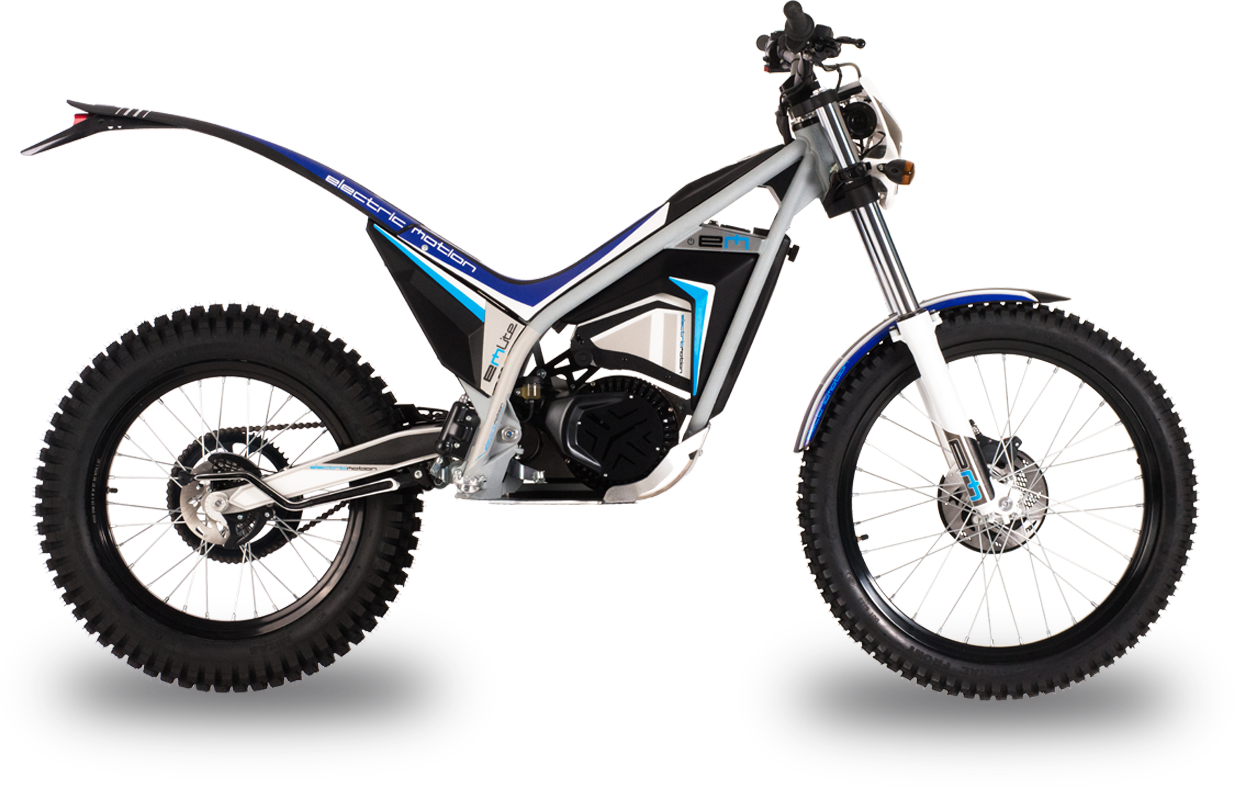
\includegraphics[width=.9\linewidth]{images/fig_01}
}%figues de la page de garde


\def\xxpied{%
Cycle 01 -- Modéliser le comportement des systèmes multiphysiques\\
\xxactivite%
}

\setcounter{secnumdepth}{5}
%---------------------------------------------------------------------------

\usepackage{pgfplots}
\begin{document}
%\defimages{images}
%\chapterimage{png/Fond_Cin}
\pagestyle{empty}


%%%%%%%% PAGE DE GARDE COURS
\ifcours
\begin{tikzpicture}[remember picture,overlay]
\node at (current page.north west)
{\begin{tikzpicture}[remember picture,overlay]
\node[anchor=north west,inner sep=0pt] at (0,0) {\includegraphics[width=\paperwidth]{\thechapterimage}};
\draw[anchor=west] (-2cm,-8cm) node [line width=2pt,rounded corners=15pt,draw=ocre,fill=white,fill opacity=0.6,inner sep=40pt]{\strut\makebox[22cm]{}};
\draw[anchor=west] (1cm,-8cm) node {\huge\sffamily\bfseries\color{black} %
\begin{minipage}{1cm}
\rotatebox{90}{\LARGE\sffamily\textsc{\color{ocre}\textbf{\xxnumpartie}}}
\end{minipage} \hfill
\begin{minipage}[c]{14cm}
\begin{titrepartie}
\begin{flushright}
\renewcommand{\baselinestretch}{1.1} 
\Large\sffamily\textsc{\textbf{\xxpartie}}
\renewcommand{\baselinestretch}{1} 
\end{flushright}
\end{titrepartie}
\end{minipage} \hfill
\begin{minipage}[c]{3.5cm}
{\large\sffamily\textsc{\textbf{\color{ocre} \discipline}}}
\end{minipage} 
 };
\end{tikzpicture}};
\end{tikzpicture}


\begin{tikzpicture}[overlay]
\node[shape=rectangle, 
      rounded corners = .25 cm,
	  draw= ocre,
	  line width=2pt, 
	  fill = ocre!10,
	  minimum width  = 2.5cm,
	  minimum height = 3cm,] at (18cm,0) {};
\node at (17.7cm,0) {\rotatebox{90}{\textbf{\Large\color{ocre}{\classe}}}};
%{};
\end{tikzpicture}

\vspace{3.5cm}

\begin{tikzpicture}[remember picture,overlay]
\draw[anchor=west] (-2cm,-6cm) node {\huge\sffamily\bfseries\color{black} %
\begin{minipage}{2cm}
\begin{center}
\LARGE\sffamily\textsc{\color{ocre}\textbf{\xxactivite}}
\end{center}
\end{minipage} \hfill
\begin{minipage}[c]{15cm}
\begin{titrechapitre}
\renewcommand{\baselinestretch}{1.1} 
\Large\sffamily\textsc{\textbf{\xxnumchapitre}}

\Large\sffamily\textsc{\textbf{\xxchapitre}}
\vspace{.5cm}

\renewcommand{\baselinestretch}{1} 
\normalsize\normalfont
\xxcompetences
\end{titrechapitre}
\end{minipage}  };
\end{tikzpicture}
\vfill

\begin{flushright}
\begin{minipage}[c]{.3\linewidth}
\begin{center}
\xxfigures
\end{center}
\end{minipage}\hfill
\begin{minipage}[c]{.6\linewidth}
\startcontents
\printcontents{}{1}{}
\end{minipage}
\end{flushright}

\begin{tikzpicture}[remember picture,overlay]
\draw[anchor=west] (4.5cm,-.7cm) node {
\begin{minipage}[c]{.2\linewidth}
\begin{flushright}

\includegraphics[width=2cm]{png/logoCC}
\end{flushright}
\end{minipage}
\begin{minipage}[c]{.2\linewidth}
\textsl{\xxauteur} \\
\textsl{\classe}
\end{minipage}
 };
\end{tikzpicture}
\newpage
\pagestyle{fancy}

\newpage
\pagestyle{fancy}

\else
\fi


%%%%%%%% PAGE DE GARDE TD
\iftd
%\begin{tikzpicture}[remember picture,overlay]
%\node at (current page.north west)
%{\begin{tikzpicture}[remember picture,overlay]
%\draw[anchor=west] (-2cm,-3.25cm) node [line width=2pt,rounded corners=15pt,draw=ocre,fill=white,fill opacity=0.6,inner sep=40pt]{\strut\makebox[22cm]{}};
%\draw[anchor=west] (1cm,-3.25cm) node {\huge\sffamily\bfseries\color{black} %
%\begin{minipage}{1cm}
%\rotatebox{90}{\LARGE\sffamily\textsc{\color{ocre}\textbf{\xxnumpartie}}}
%\end{minipage} \hfill
%\begin{minipage}[c]{13.5cm}
%\begin{titrepartie}
%\begin{flushright}
%\renewcommand{\baselinestretch}{1.1} 
%\Large\sffamily\textsc{\textbf{\xxpartie}}
%\renewcommand{\baselinestretch}{1} 
%\end{flushright}
%\end{titrepartie}
%\end{minipage} \hfill
%\begin{minipage}[c]{3.5cm}
%{\large\sffamily\textsc{\textbf{\color{ocre} \discipline}}}
%\end{minipage} 
% };
%\end{tikzpicture}};
%\end{tikzpicture}

%%%%%%%%%% PAGE DE GARDE TD %%%%%%%%%%%%%%%
%\begin{tikzpicture}[overlay]
%\node[shape=rectangle, 
%      rounded corners = .25 cm,
%	  draw= ocre,
%	  line width=2pt, 
%	  fill = ocre!10,
%	  minimum width  = 2.5cm,
%	  minimum height = 2.5cm,] at (18.5cm,0) {};
%\node at (17.7cm,0) {\rotatebox{90}{\textbf{\Large\color{ocre}{\classe}}}};
%%{};
%\end{tikzpicture}

% PARTIE ET CHAPITRE
%\begin{tikzpicture}[remember picture,overlay]
%\draw[anchor=west] (-1cm,-2.1cm) node {\large\sffamily\bfseries\color{black} %
%\begin{minipage}[c]{15cm}
%\begin{flushleft}
%\xxnumchapitre \\
%\xxchapitre
%\end{flushleft}
%\end{minipage}  };
%\end{tikzpicture}

% Bandeau titre exo
\begin{tikzpicture}[remember picture,overlay]
\draw[anchor=west] (-2cm,-6cm) node {\huge\sffamily\bfseries\color{black} %
\begin{minipage}{5cm}
\begin{center}
\LARGE\sffamily\color{ocre}\textbf{\textsc{\xxactivite}}

\begin{center}
\xxfigures
\end{center}

\end{center}
\end{minipage} \hfill
\begin{minipage}[c]{12cm}
\begin{titrechapitre}
\renewcommand{\baselinestretch}{1.1} 
\large\sffamily\textbf{\textsc{\xxtitreexo}}

\small\sffamily{\textbf{\textit{\color{black!70}\xxsourceexo}}}
\vspace{.5cm}

\renewcommand{\baselinestretch}{1} 
\normalsize\normalfont
\xxcompetences
\end{titrechapitre}
\end{minipage}  };
\end{tikzpicture}

\else
\fi


%%%%%%%% PAGE DE GARDE FICHE
\iffiche
\begin{tikzpicture}[remember picture,overlay]
\node at (current page.north west)
{\begin{tikzpicture}[remember picture,overlay]
\draw[anchor=west] (-2cm,-3.25cm) node [line width=2pt,rounded corners=15pt,draw=ocre,fill=white,fill opacity=0.6,inner sep=40pt]{\strut\makebox[22cm]{}};
\draw[anchor=west] (1cm,-3.25cm) node {\huge\sffamily\bfseries\color{black} %
\begin{minipage}{1cm}
\rotatebox{90}{\LARGE\sffamily\textsc{\color{ocre}\textbf{\xxnumpartie}}}
\end{minipage} \hfill
\begin{minipage}[c]{14cm}
\begin{titrepartie}
\begin{flushright}
\renewcommand{\baselinestretch}{1.1} 
\large\sffamily\textsc{\textbf{\xxpartie} \\} 

\vspace{.2cm}

\normalsize\sffamily\textsc{\textbf{\xxnumchapitre -- \xxchapitre}}
\renewcommand{\baselinestretch}{1} 
\end{flushright}
\end{titrepartie}
\end{minipage} \hfill
\begin{minipage}[c]{3.5cm}
{\large\sffamily\textsc{\textbf{\color{ocre} \discipline}}}
\end{minipage} 
 };
\end{tikzpicture}};
\end{tikzpicture}


\begin{tikzpicture}[overlay]
\node[shape=rectangle, 
      rounded corners = .25 cm,
	  draw= ocre,
	  line width=2pt, 
	  fill = ocre!10,
	  minimum width  = 2.5cm,
%	  minimum height = 2.5cm,] at (18.5cm,0.5cm) {};
	  minimum height = 2.5cm,] at (18.5cm,0cm) {};
\node at (17.7cm,0) {\rotatebox{90}{\textsf{\textbf{\large\color{ocre}{\classe}}}}};
%{};
\end{tikzpicture}



\else
\fi



\vspace{4cm}
\pagestyle{fancy}
\thispagestyle{plain}
\def\pathfig{images2}
\def\columnseprulecolor{\color{ocre}}
\setlength{\columnseprule}{0.4pt} 

%\defimages2{images}

%\begin{multicols}{2}
%%%%%%%%%%%%%%%%%%%%%%%%%%%%%%%%%%%%%
\section{Détermination des performances d'un système de téléchirurgie robotisée au contact d'organes mobiles.}


\noindent \begin{minipage}[c]{.6\linewidth}

 La téléopération consiste à utiliser deux dispositifs robotisés, le robot-maître est manœuvré par le chirurgien et le robot-esclave est au contact de l'organe à opérer.
%Une première phase de modélisation a été menée et
%différentes exigences ont déjà été validées au cours de l'exercice A du chapitre 1.

\textbf{Cahier des charges\\}
Les exigences validées précédemment sont représentées sur la figure ci-dessous.

\end{minipage} \hfill
\begin{minipage}[c]{.4\linewidth}
\begin{center}
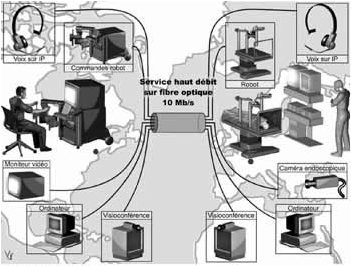
\includegraphics[width=.9\textwidth]{\pathfig/Sup.png}

\end{center}
\end{minipage}


\begin{center}%[!ht]
%\centering
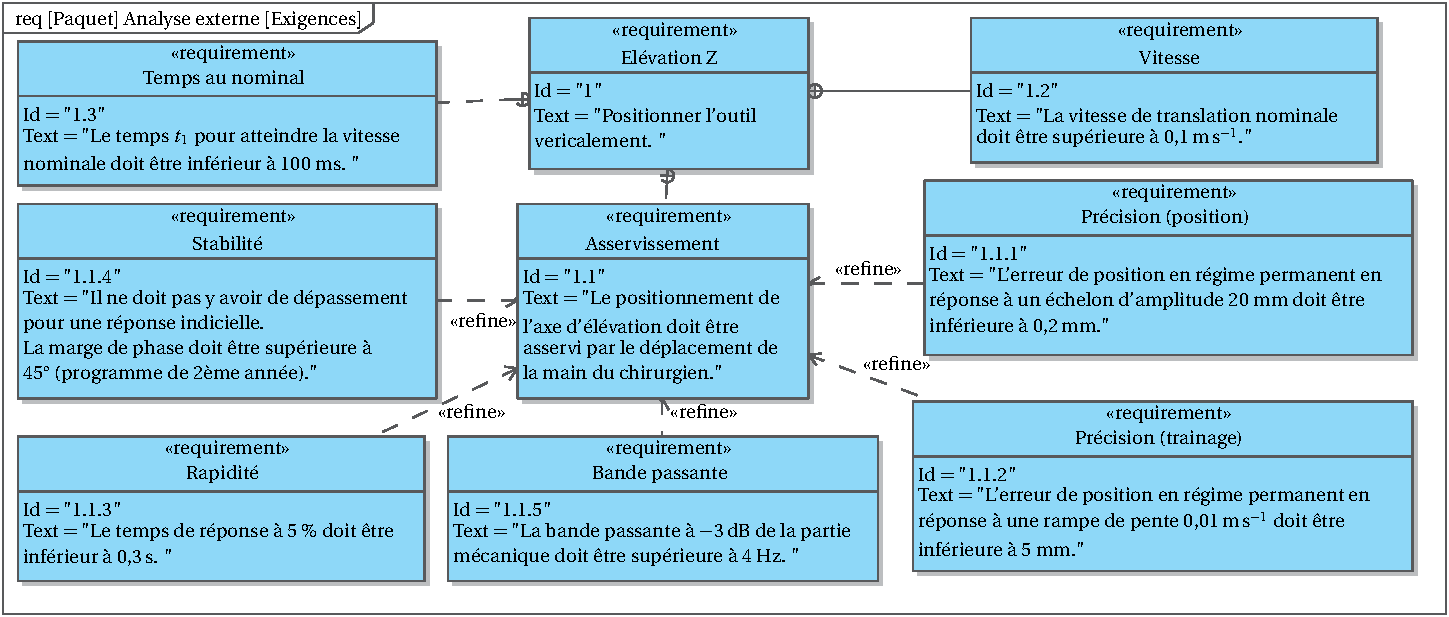
\includegraphics[width=.9\textwidth]{\pathfig/Diagramme_exigences}

\textit{Diagramme des exigences partiel.}
\label{chap2:tele:req}
\end{center}




\subsubsection*{Problème posé}
\begin{obj}
Le modèle du système a été mis en place précédemment. L'objectif de cette étude est de concevoir et valider une commande permettant de
rejeter une perturbation périodique. 
\end{obj}



\subsection{Modéliser la commande}


La modélisation de la commande est donnée par le schéma-blocs figure suivante.% \ref{chap2:tele:complet}.


%\begin{figure}[!ht]
\begin{center}
%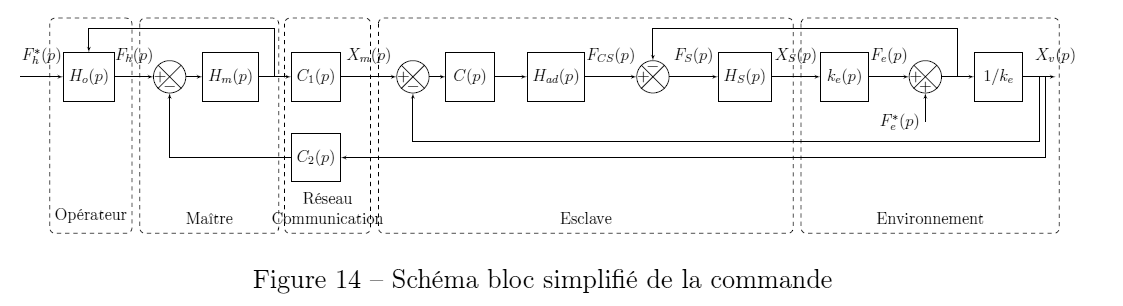
\includegraphics[width=1.\textwidth]{\pathfig/T10}
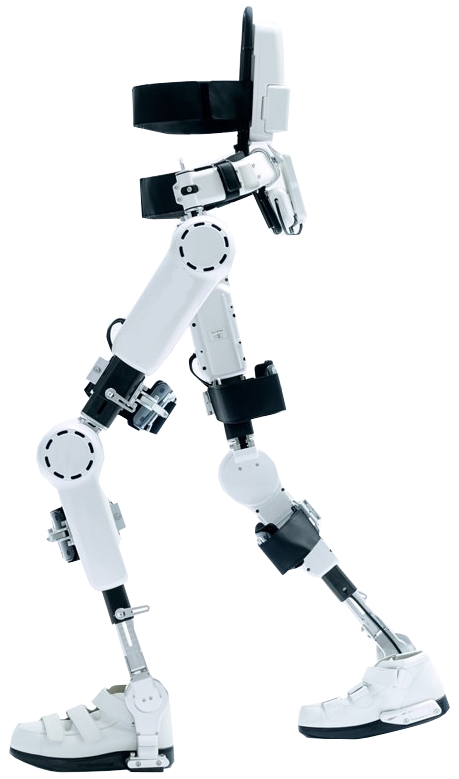
\includegraphics[width=\textwidth]{\pathfig/fig_01}
%\resizebox{\linewidth}{!}{
%\begin{tikzpicture}[every node/.style={scale=1.27}]
%\sbEntree{E}
%\sbBlocL[3]{Ho}{$H_o(p)$}{E}
%\sbComp[5]{Comp1}{Ho}
%\sbRelier{Ho}{Comp1}
%\sbBlocL[1]{Hm}{$H_m(p)$}{Comp1}
%\sbBlocL{C1}{$C_1(p)$}{Hm}
%\sbComp[6]{Comp2}{C1}
%\sbRelier{C1}{Comp2}
%\sbBlocL[1]{C}{$C(p)$}{Comp2}
%\sbBlocL{Had}{$H_{ad}(p)$}{C}
%\sbComph[6]{Comp3}{Had}
%\sbRelier{Had}{Comp3}
%\sbBlocL[3]{Hs}{$H_S(p)$}{Comp3}
%\sbBlocL[3]{ke}{$k_e(p)$}{Hs}
%\sbSumb[5]{Comp4}{ke}
%\sbRelier{ke}{Comp4}
%\sbBlocL{1ke}{$1/k_e$}{Comp4}
%\sbSortie{S}{1ke}
%\sbRelier{1ke}{S}
%\draw[->,>=latex'] (Hm-C1.south) -- ++(0,3em) -| (Ho);
%\sbRenvoi[-3]{Comp4-1ke}{Comp3}{}
%\sbRenvoi{1ke-S}{Comp2}{}
%\sbDecaleNoeudy[5]{C1droite}{C2d}
%\sbBlocr[0]{C2}{$C_2(p)$}{C2d}
%\draw[->,>=latex'] ($(1ke-S.south)+(1.5mm,0)$) |- (C2);
%\sbRelierxy{C2}{Comp1}
%
%\node[yshift=3ex] at (E-Ho.south) {$F_h^*(p)$};
%\node[yshift=3ex,xshift=.4mm-1pt] at (Ho-Comp1.south) {$F_h(p)$};
%\node[yshift=3ex] at (C1-Comp2.south) {$X_m(p)$};
%\node[yshift=3ex] at (Had-Comp3.south) {$F_{CS}(p)$};
%\node[yshift=3ex] at (Comp3-Hs.south) {$F_{S}(p)$};
%\node[yshift=3ex] at (Hs-ke.south) {$X_{S}(p)$};
%\node[yshift=3ex] at (ke-Comp4.south) {$F_e(p)$};
%\draw[<-,>=latex'] (Comp4.south) -- ++(0,-4ex) node[left] {$F_e^*(p)$};
%\node[yshift=3ex] at (S.south) {$X_v(p)$};
%
%\draw[rounded corners=4pt,dashed] (0.9,1.5) rectangle (3,-4) node[midway,align=center,yshift=-2.cm,anchor=south,inner sep=0pt,outer sep=0pt] {Opérateur};
%\draw[rounded corners=4pt,dashed] (3.2,1.5) rectangle (6.75,-4) node[midway,align=center,yshift=-2.cm,anchor=south,inner sep=0pt,outer sep=0pt] {Maître};
%\draw[rounded corners=4pt,dashed] (6.9,1.5) rectangle (9.1,-4) node[midway,align=center,yshift=-2.cm,anchor=south,inner sep=0pt,outer sep=0pt] {Réseau\\Communication};
%\draw[rounded corners=4pt,dashed] (9.3,1.5) rectangle (19.9,-4) node[midway,align=center,yshift=-2.cm,anchor=south,inner sep=0pt,outer sep=0pt] {Esclave};
%\draw[rounded corners=4pt,dashed] (20.1,1.5) rectangle (26.7,-4) node[midway,align=center,yshift=-2.cm,anchor=south,inner sep=0pt,outer sep=0pt] {Environnement};
%\end{tikzpicture}}
\textit{Schéma-blocs simplifié de la commande. \label{chap2:tele:complet}}
%\caption{Schéma-blocs simplifié de la commande. \label{chap2:tele:complet}}
%\end{figure}
\end{center}

Ainsi, la modélisation permettant de relier la consigne $x_m(t)$ issue du dispositif-maître au déplacement
$x_v(t)$ de l'organe terminal est représentée par le schéma-blocs suivant.%de la figure \ref{chap2:tele:bloc1}.

%\begin{figure}[!ht]
\begin{center}
%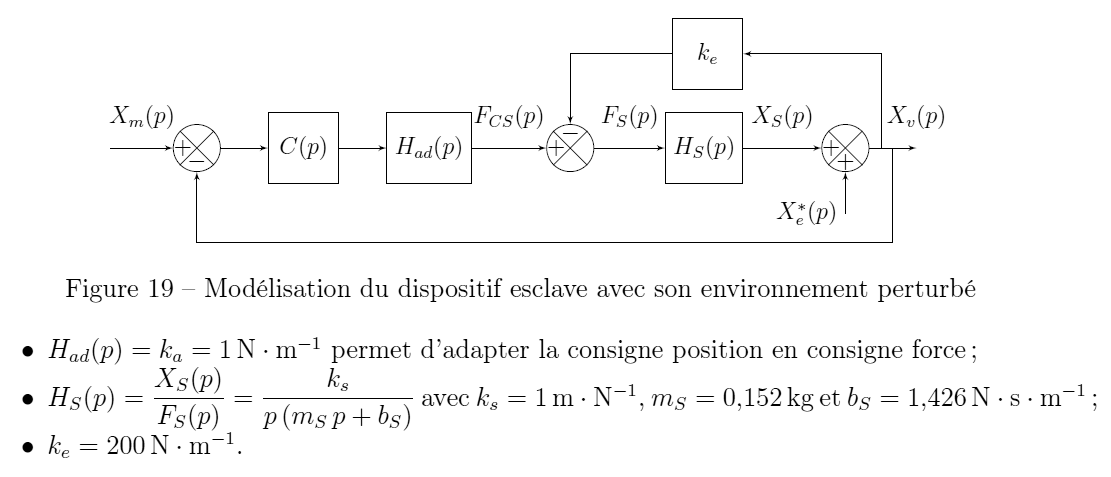
\includegraphics[width=.7\textwidth]{\pathfig/T16.png}
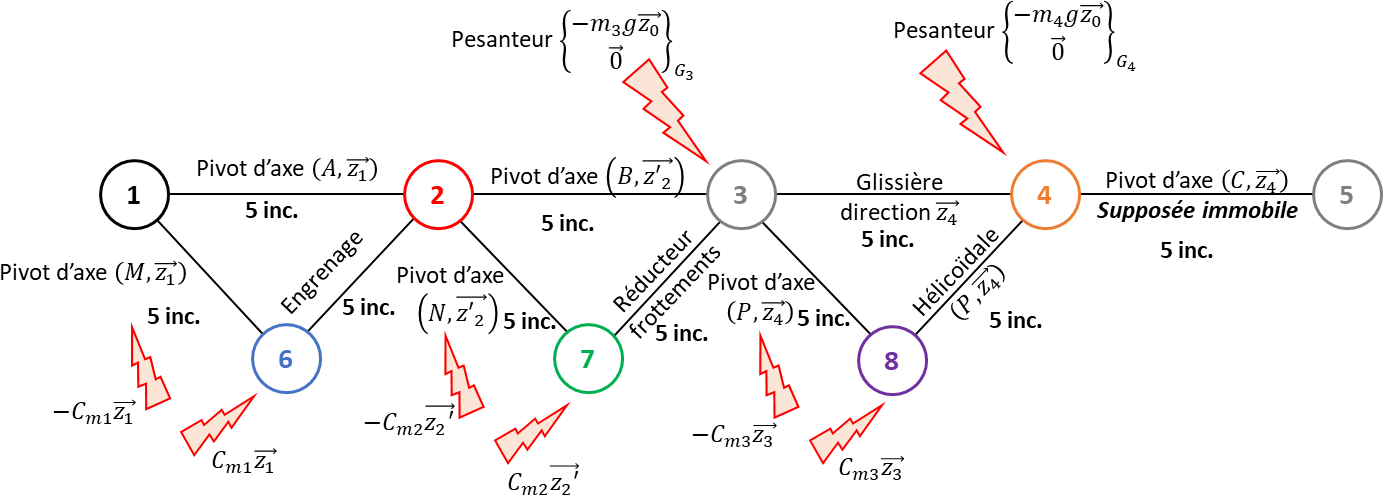
\includegraphics[width=.7\textwidth]{\pathfig/fig_02}
%\scalebox{.7}{
%\begin{tikzpicture}
%\sbEntree{E}
%\sbComp{Comp1}{E}
%\sbRelier{E}{Comp1}
%\sbBlocL{C}{$C(p)$}{Comp1}
%\sbBlocL{Had}{$H_{ad}(p)$}{C}
%\sbComph[6]{Comp2}{Had}
%\sbRelier{Had}{Comp2}
%\sbBlocL[3]{Hs}{$H_S(p)$}{Comp2}
%\sbSumb[6]{Comp3}{Hs}
%\sbRelier{Hs}{Comp3}
%\sbSortie{S}{Comp3}
%\sbRelier{Comp3}{S}
%\sbRenvoi{Comp3-S}{Comp1}{}
%\sbDecaleNoeudy[-4]{Hsdroite}{ke1}
%\sbBlocr[0]{ke}{$k_e$}{ke1}
%\draw[->,>=latex'] ($(Comp3-S.south)+(-2mm,0)$) |- (ke);
%\sbRelierxy{ke}{Comp2}
%
%\node[yshift=3ex] at (E-Comp1.south) {$X_m(p)$};
%\node[yshift=3ex] at (Had-Comp2.south) {$F_{CS}(p)$};
%\node[yshift=3ex] at (Comp2-Hs.south) {$F_{S}(p)$};
%\node[yshift=3ex] at (Hs-Comp3.south) {$X_{S}(p)$};
%\draw[<-,>=latex'] (Comp3.south) -- ++(0,-4ex) node[left] {$X_e^*(p)$};
%\node[yshift=3ex] at (S.south) {$X_v(p)$};
%
%\end{tikzpicture}}
%\textit{Modélisation du dispositif esclave avec son environnement perturbé.
%\label{chap2:tele:bloc1}}

%\caption{Modélisation du dispositif esclave avec son environnement perturbé.
%\label{chap2:tele:bloc1}}
%\end{figure}
\end{center}

%\FloatBarrier
On a :
\begin{itemize}
\item $H_{ad}(p) = k_a = \SI{1}{N.m^{-1}}$ permet d'adapter la consigne position en consigne force;
\item  $H_S(p) = \frac{X_S(p)}{F_S(p)}= \frac{k_s}{p\left( m_S \, p + b_S\right) }$ avec $k_s = \SI{1}{m.N^{-1}}$, $m_S = \SI{0,152}{kg}$ et $b_S = \SI{1,426}{N.s.m^{-1}}$;
\item $k_e = \SI{200}{N.m^{-1}}$.
\end{itemize}



\subparagraph{}\textit{Simplifier le schéma-blocs précédent pour lui donner la forme illustrée par la figure suivante. 
Exprimer $H_t(p)$ et $H(p)$ en fonction de $k_e$, $k_a$ et $H_s(p)$.
}

%\interenum{
%\begin{figure}[!ht]
\begin{center}
%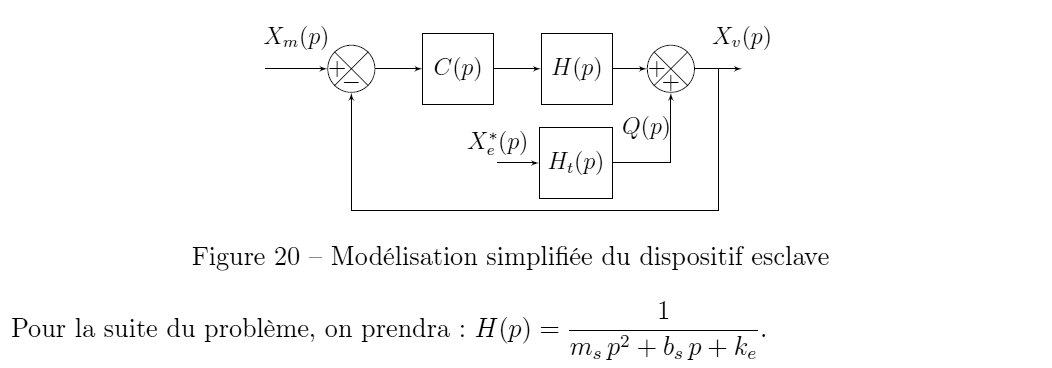
\includegraphics[width=.7\textwidth]{\pathfig/T17.png}
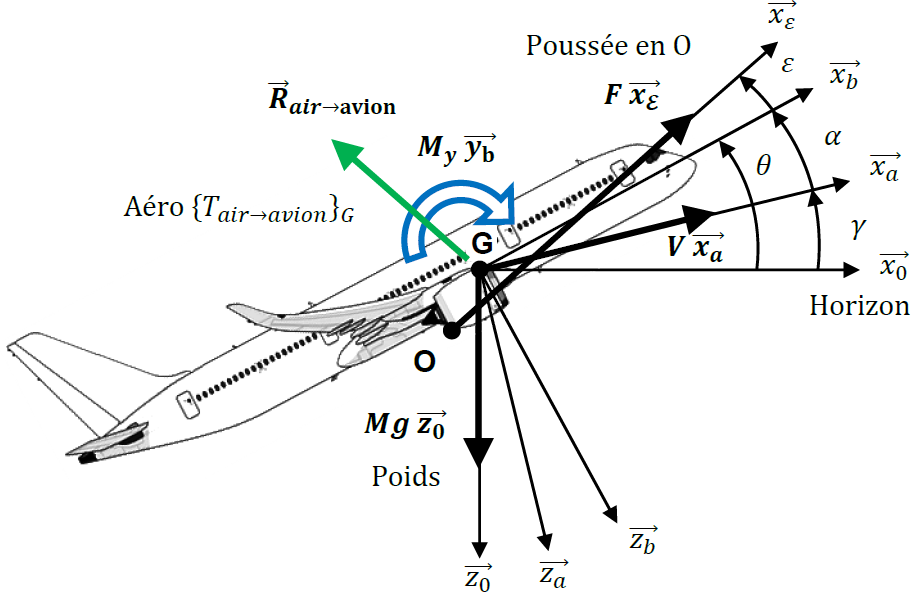
\includegraphics[width=.5\textwidth]{\pathfig/fig_03.png}
%
%\scalebox{.7}{
%\begin{tikzpicture}
%\sbEntree{E}
%\sbComp{Comp1}{E}
%\sbRelier{E}{Comp1}
%\sbBlocL{C}{$C(p)$}{Comp1}
%\sbBlocL{H}{$H(p)$}{C}
%\sbSumb{Comp2}{H}
%\sbRelier{H}{Comp2}
%\sbSortie{S}{Comp2}
%\sbRelier{Comp2}{S}
%\sbRenvoi[6]{Comp2-S}{Comp1}{}
%\sbDecaleNoeudy[4]{Hdroite}{ht1}
%\sbBlocr[0]{ht}{$H_t(p)$}{ht1}
%\sbRelierxy{ht}{Comp2}
%
%\node[left] at (ht-Comp2) {$Q(p)$};
%\node[yshift=3ex] at (E-Comp1.south) {$X_m(p)$};
%\draw[<-,>=latex'] (ht.west) -- ++(-4ex,0) node[above] {$X_e^*(p)$};
%\node[yshift=3ex] at (S.south) {$X_v(p)$};
%
%\end{tikzpicture}}

\textit{Modélisation simplifiée du dispositif-esclave.}
%\caption{Modélisation simplifiée du dispositif-esclave.
%\label{chap2:tele:bloc2}}
\end{center}

Pour la suite du problème, on prendra $ H(p)= \frac{1}{m_S p^2 +b_S p+ k_e}$.


\subsection{Caractériser les performances du système sans correction : $C(p) = 1$\\}

L'objectif de cette partie est d'identifier les performances non satisfaites afin de choisir un correcteur adapté.



\subparagraph{}\textit{Déterminer la fonction de transfert en boucle fermée (avec une perturbation nulle :
$X_e^*(p) =0$) : $F_{BF1}(p) = \frac{ X_v(p)}{ X_m(p)}$, puis la mettre sous forme canonique de façon à identifier
les paramètres caractéristiques : gain statique ($K$), pulsation propre ($\omega_0$) et coefficient d'amortissement
($z$). Faire l'application numérique.}

%\begin{figure}[!ht]
%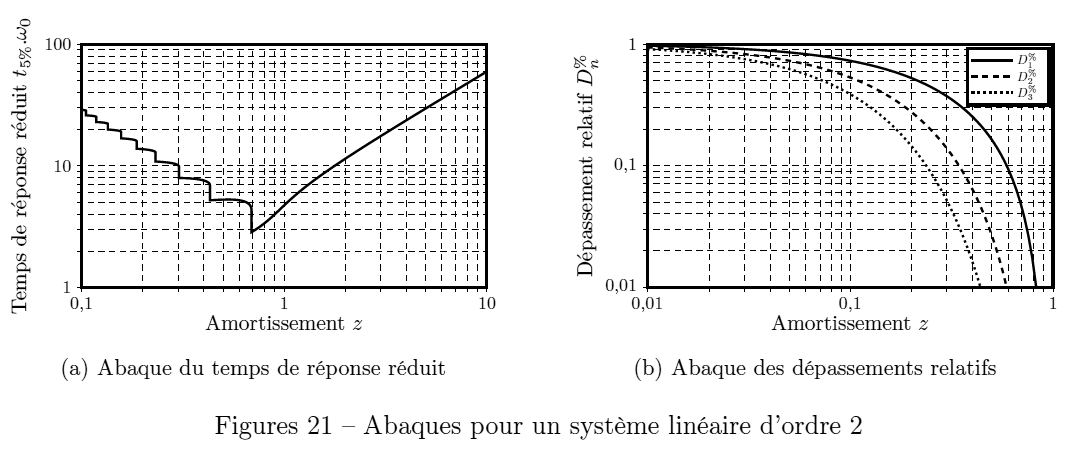
\includegraphics[width=.7\textwidth]{\pathfig/T18.png}
\begin{minipage}[c]{.47\linewidth}
\begin{center}
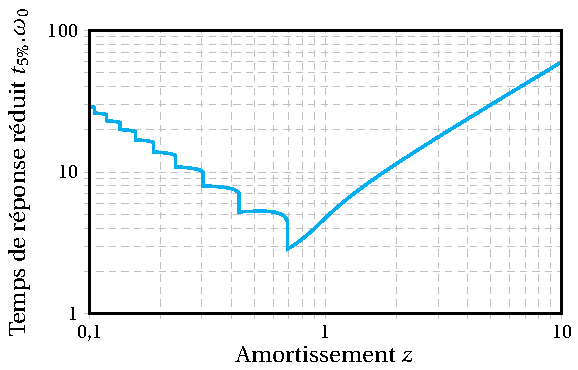
\includegraphics[width=8cm]{\pathfig/figure5}

\textit{Abaque du temps de réponse réduit}
\end{center}
\end{minipage} \hfill
\begin{minipage}[c]{.47\linewidth}
\begin{center}
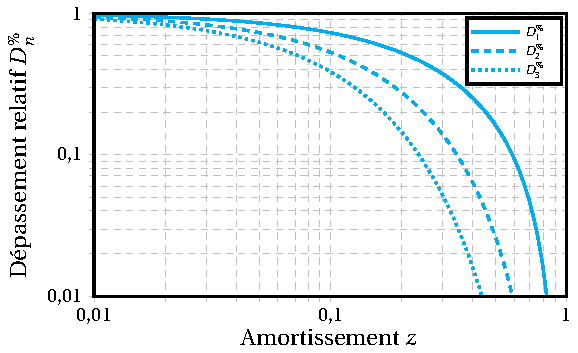
\includegraphics[width=8cm]{\pathfig/figure6}

\textit{Abaque des dépassements relatifs}
\end{center}
\end{minipage}
%\subfigure[Abaque du temps de réponse réduit\label{abaque_tempsreponse}]%{\includesgraphics[width=5.5cm]{\pathfig/figure5}}\hfill
%\subfigure[Abaque des dépassements relatifs\label{abaque_depassement}]{\includesgraphics[width=5.5cm]{\pathfig/figure6}}


%\caption{Abaques pour un système linéaire d'ordre 2.
%\label{chap2:tele:abaque}}
%\vspace*{-1em}
%\end{figure}


\subparagraph{}\textit{En vous aidant des abaques de la figure précédente, vérifier les exigences « stabilité »
(uniquement l'amortissement), « rapidité » et « précision » (uniquement l'erreur statique).}
%\ref{chap2:tele:abaque}


\subsection{Caractériser les performances du système avec
correction intégrale : $C(p)=\frac{K_i}{p}$\\}


L'objectif est de vérifier la capacité d'une correction intégrale à atteindre les exigences.


\subparagraph{}\textit{Les résultats d'une simulation pour un gain $K_i = 100$ sont donnés sur le document réponse. Vérifier les exigences « stabilité », « rapidité », « précision » (uniquement l'erreur statique)
et compléter le tableau.}

%\newpage
%
%
%\begin{center}%[!ht]
%%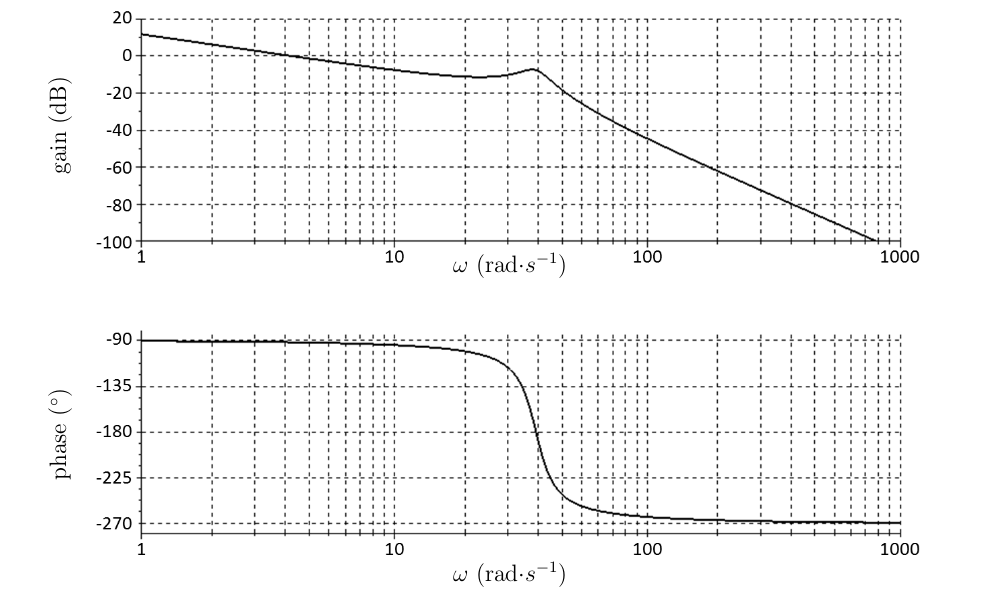
\includegraphics[width=.7\textwidth]{\pathfig/DR1.png}
%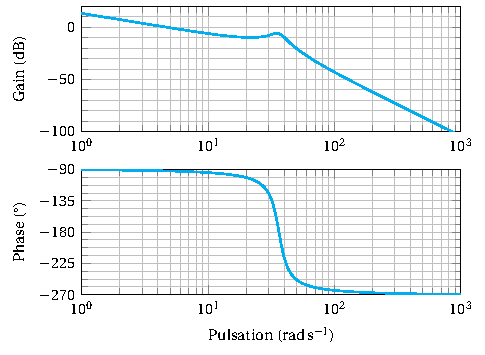
\includegraphics[width=.8\linewidth]{\pathfig/systeme_corrige_bode}
%
%\textit{Diagramme de Bode de la fonction de transfert en boucle ouverte pour $K_i = 100$.}
%%\caption{Diagramme de Bode de la fonction de transfert en boucle ouverte pour $K_i = 100$.
%%\label{chap2:tele:DR1}}
%\end{center}
%
%%\begin{figure}[!ht]
%%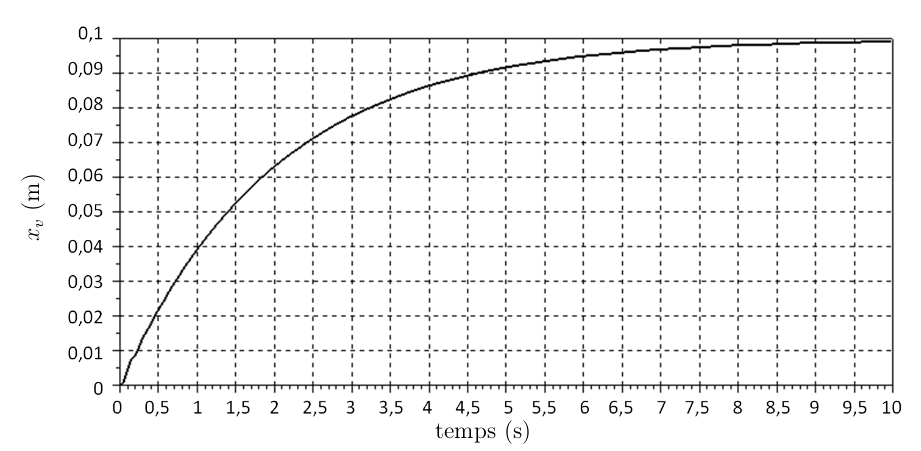
\includegraphics[width=.7\textwidth]{\pathfig/DR1bis.png}
%\begin{center}
%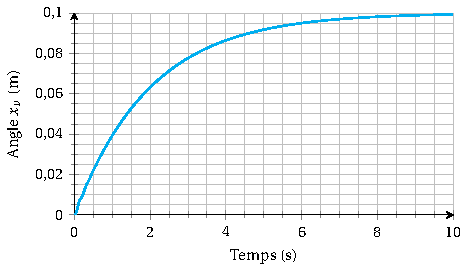
\includegraphics{\pathfig/systeme_corrige_reponse}
%
%\textit{Réponse temporelle de la fonction de transfert en boucle fermée pour un échelon de $\SI{10}{cm}$ et
%$K_i = 100$.
%\label{chap2:tele:DR1bis}}
%%\end{figure}
%\end{center}
%
%
%%\begin{figure}[!ht]
%%\begin{footnotesize}
%\begin{center}
%\begin{tabular}{|l|p{3cm}|}
%\hline 
%\textbf{Temps de réponse à 5 \%} &\\
%\hline
%\textbf{Amplitude du premier dépassement} &\\
%\hline
%\textbf{Erreur statique} &\\
%\hline
%\textbf{Marge de phase} &\\
%\hline
%\textbf{Marge de gain}&\\
%\hline
%\end{tabular} 
%%\end{footnotesize}
%
%\textit{Performance de l'asservissement avec correction PI et $K_i = 100$.
%\label{chap2:tele:DR1ter}}
%\end{center}
%

\subparagraph{}\textit{Pour améliorer la rapidité, il faut augmenter le gain $K_i$. Déterminer la valeur $K_{\text{imax}}$ du
coefficient $K_i$ qui permet de respecter les deux marges de stabilité.}



\subparagraph{}\textit{En analysant la courbe du document réponse, compléter le tableau puis conclure sur la capacité du correcteur à valider simultanément les exigences
de « stabilité » et de « rapidité ».
}
%
%
%%\interenum{
%\begin{center}%[!ht]
%%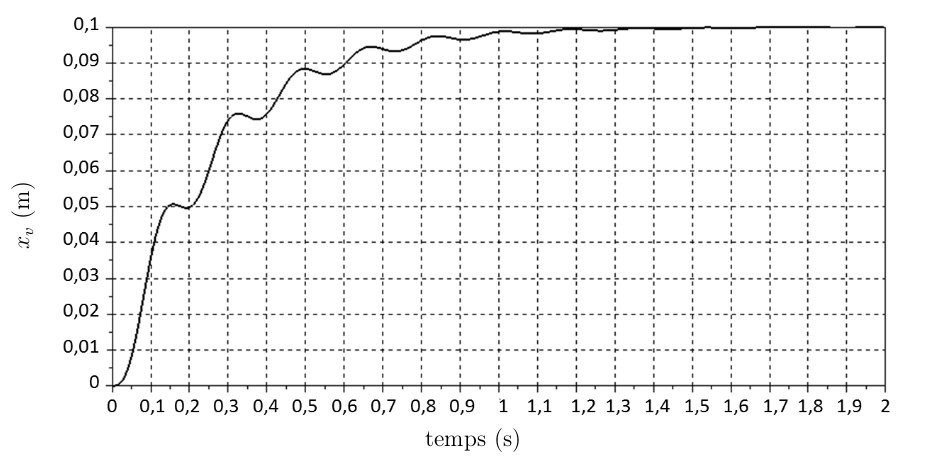
\includegraphics[width=.7\textwidth]{\pathfig/DR2.png}
%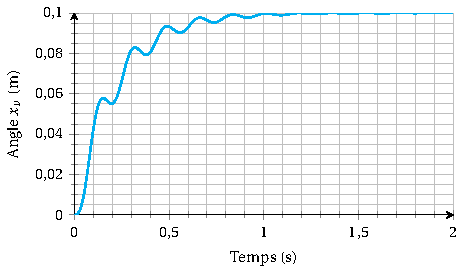
\includegraphics{\pathfig/systeme_corrige_reponse_opti}
%
%\textit{Réponse temporelle de la fonction de transfert en boucle fermée pour un échelon de $\SI{10}{cm}$
%avec le réglage $K_{\text{imax}}$.
%\label{chap2:tele:DR2}}
%\end{center}
%
%\begin{center}%[!ht]
%%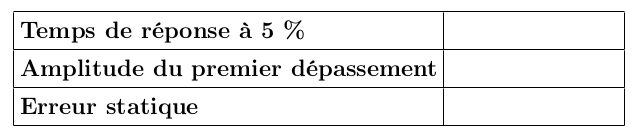
\includegraphics[width=.7\textwidth]{\pathfig/DR2bis.png}
%%\begin{footnotesize}
%\begin{tabular}{|l|p{3cm}|}
%\hline 
%\textbf{Temps de réponse à 5~\%} &\\
%\hline
%\textbf{Amplitude du premier dépassement} &\\
%\hline
%\textbf{Erreur statique} &\\ 
%\hline
%\end{tabular} 
%%\end{footnotesize}
%
%\textit{Performance de l'asservissement avec correction PI et $K_i = K_{\text{imax}}$.
%\label{chap2:tele:DR2bis}}
%\end{center}
%
%
%


\subparagraph{}\textit{Le diagramme de Bode de la figure suivante représente la réponse fréquentielle (courbe de gain
uniquement) de la fonction $F_{BF2}(j \omega) = \frac{X_v(j \omega)}{X_e^*(j \omega)}$ pour $K_i = K_{\text{imax}}$. Quelle sera l'atténuation minimale $|F_{BF2}(j \omega)|_{\text{min}}$ de la perturbation $x_e^*$
(en $\%$) sur l'intervalle $[\SI{1,25}{rad.s^{-1}}; \SI{12,5}{rad.s^{-1}}]$.
Conclure sur la validation de l'exigence de « précision ».}



\begin{center}%[!ht]
%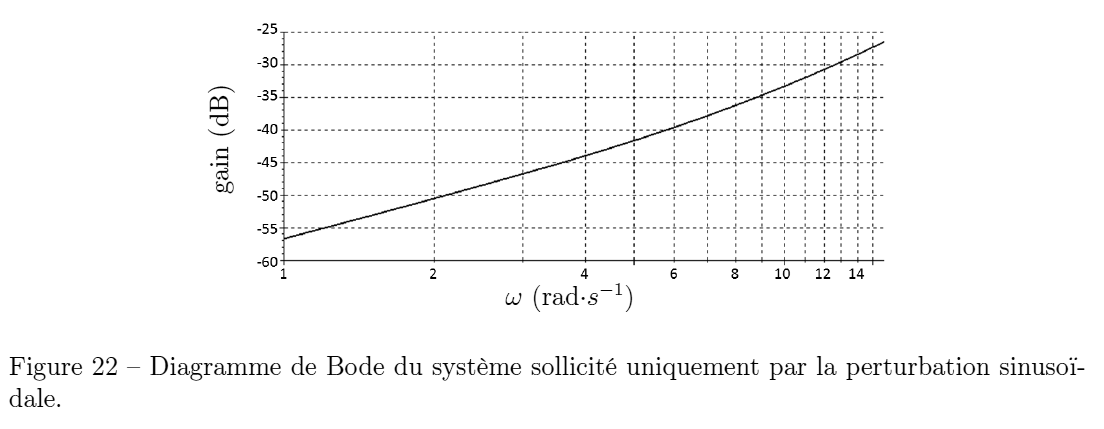
\includegraphics[width=.7\textwidth]{\pathfig/T19.png}

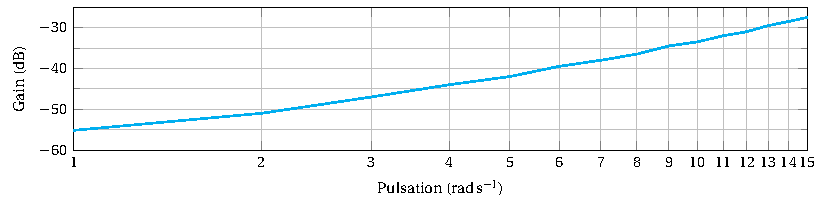
\includegraphics[scale=.8]{\pathfig/systeme_corrige_bode_opti}

\textit{Diagramme de Bode du système sollicité uniquement par la perturbation sinusoïdale.
\label{chap2:tele:19}}
\end{center}

\subsection{Caractériser les performances du système avec correction IMC}

L'objectif est d'améliorer la rapidité tout en atténuant la perturbation sinusoïdale.


Pour améliorer l'atténuation de la perturbation sinusoïdale, il est possible de changer la
structure de l'asservissement et d'opter pour une correction IMC (Internal Model Corrector)
dont le schéma-blocs est donné ci-dessous.%sur la figure \ref{chap2:tele:20}.

\begin{center}%[!ht]
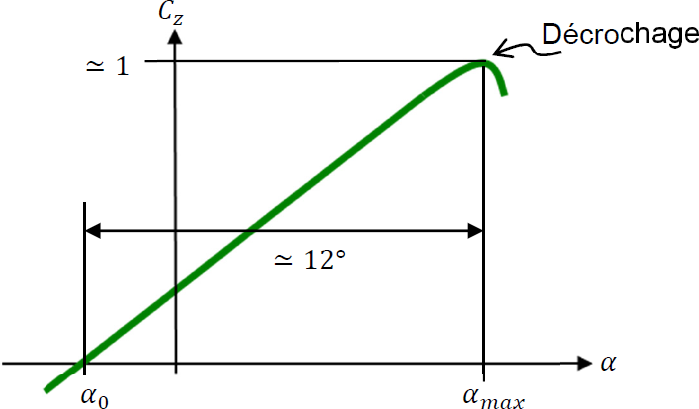
\includegraphics[width=.7\textwidth]{\pathfig/fig_04.png}

%\scalebox{.6}{
%\begin{tikzpicture}[every node/.style={scale=1.27}]
%\sbEntree{E}
%\sbComp{Comp1}{E}
%\sbRelier{E}{Comp1}
%\sbBlocL{1H}{$1/H(p)$}{Comp1}
%\sbBlocL{F}{$F(p)$}{1H}
%\sbBlocL{H1}{$H(p)$}{F}
%\sbSumb[12]{Comp2}{H1}
%\sbRelier{H1}{Comp2}
%\sbSortie{S}{Comp2}
%\sbRelier{Comp2}{S}
%\sbDecaleNoeudy{Comp2}{Ht1}
%\sbBlocr{Ht}{$H_t(p)$}{Ht1}
%\sbRelierxy{Ht}{Comp2}
%\draw[<-,>=latex'] (Ht.west) -- ++(-4ex,0) node[above] {$X_e^*(p)$};
%
%\sbDecaleNoeudy{H1droite}{H2d}
%\sbBlocr[0]{H2}{$H(p)$}{H2d}
%\sbRelieryx{F-H1}{H2}
%
%\coordinate (C3) at ($(H2d)+(2em,-3em)$) ;
%\sbCompSum[0]{Comp3}{C3}{-}{}{}{+}
%\sbRelierxy{H2}{Comp3}
%\sbRelieryx{Comp2-S}{Comp3}
%\sbRelierxy{Comp3}{Comp1}
%
%\node[left] at (Ht-Comp2) {$Q(p)$};
%\node[yshift=3ex] at (E-Comp1.south) {$X_m(p)$};
%\node[yshift=3ex] at (S.south) {$X_v(p)$};
%
%\draw[dashed] (2.5,1.) rectangle (6.8,-1.) node[midway,yshift=-1.cm,below] {$C(p)$};
%\end{tikzpicture}}

\textit{Modélisation avec correcteur IMC.
\label{chap2:tele:20}}
\end{center}


Avec $F(p)$ la fonction de transfert d'un filtre de la forme $F(p)=\frac{1}{(1+T p)^2}$ et la fonction de transfert $H(p)= \frac{1}{m_S p^2 + b_S p + k_e}$.

La grandeur de sortie $X_v(p)$ peut s'exprimer par l'équation:

$X_v(p)=A(p) X_m(p) + B(p) Q(p)$ avec $A(p)=\frac{1}{(1+T p)^2}$ et $B(p)=\frac{T p (2 + T p)}{(1+T p)^2}$.



\subparagraph{}\textit{Indiquer s'il faut augmenter ou diminuer la valeur de $T$ pour améliorer le temps de réponse
consécutif à un échelon de consigne $x_m(t) = x_0$ (on prendra $Q(p) = 0$ pour cette question).
Justifier votre réponse. En déduire la valeur limite de $T$ permettant de satisfaire l'exigence de
« rapidité ».}

\begin{center}%[!ht]
%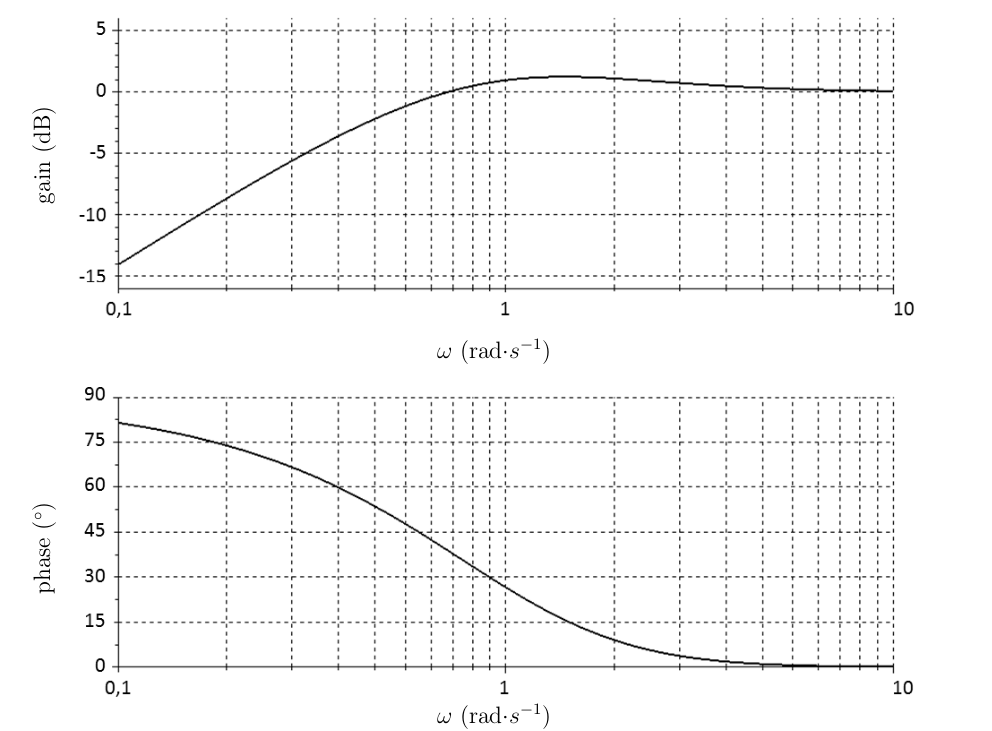
\includegraphics[width=.7\textwidth]{\pathfig/DR3.png}

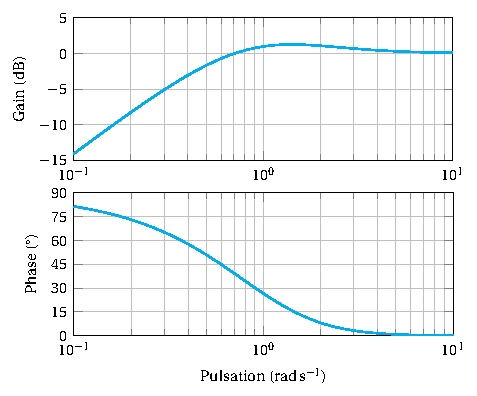
\includegraphics[scale=1.2]{\pathfig/systeme_b}

\textit{Réponse fréquentielle de $B(j\omega)$.
\label{chap2:tele:DR3}}
\end{center}

\subparagraph{}\textit{Le diagramme de Bode de $B(j \omega)$ pour $T = \SI{1}{s}$ est donné ci-dessus.
Indiquer s'il faut augmenter ou diminuer la valeur de $T$ pour minimiser l'effet de
la perturbation sur l'intervalle $[\SI{1,25}{rad.s^{-1}}; \SI{12,5}{rad.s^{-1}}]$. Justifier votre réponse. En déduire
la valeur limite de $T$ permettant de satisfaire l'atténuation de la perturbation liée à l'exigence
de « précision » sur cet intervalle.}


\subsubsection*{Retour sur le cahier des charges}

%\begin{enumerate}[label=\arabic*),start=10]

\subparagraph{}\textit{Les courbes figure suivante montrent la réponse mesurée sur la maquette et
le résultat provenant du calcul sur le modèle obtenu. Conclure sur les écarts.} 
%\end{enumerate}

\begin{center}
%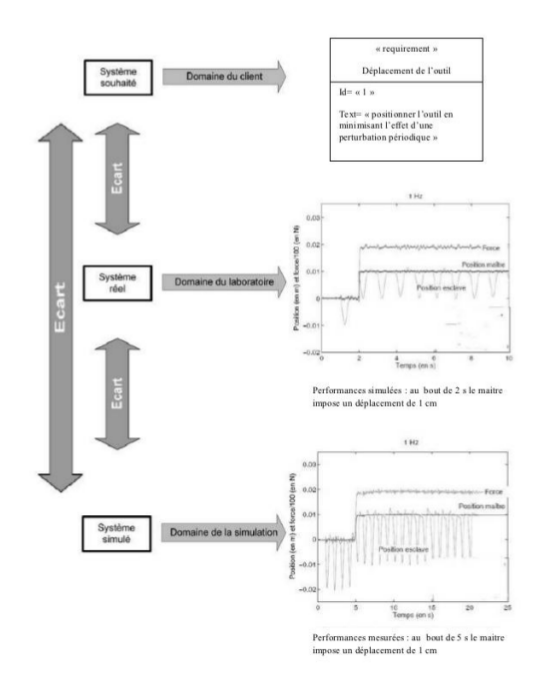
\includegraphics[width=.7\textwidth]{\pathfig/conclusion.png}
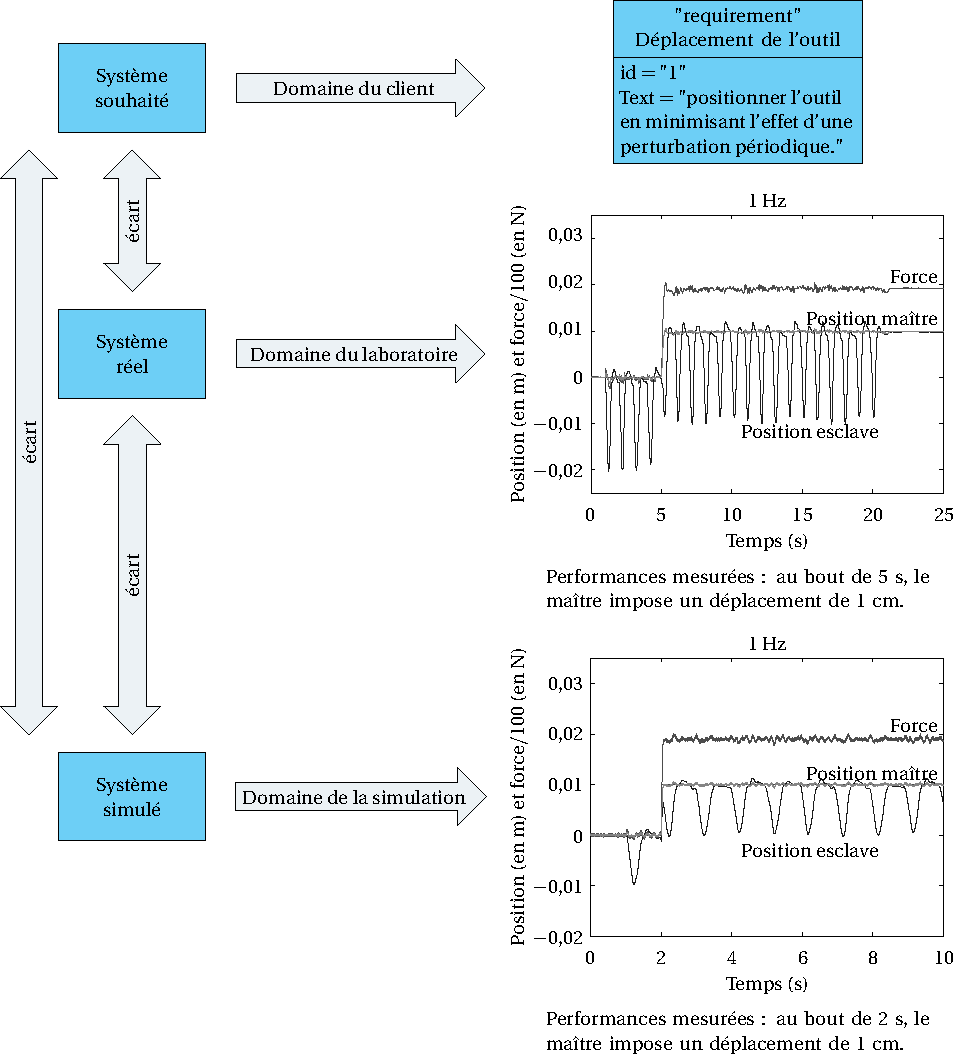
\includegraphics[width=.8\textwidth]{images2/bilan}

\textit{Synthèse.
\label{chap2:tele:DR4}}
\end{center}




%%%%%%%%%%%%%%%%%%%%%%%%%%%%%%%%%%%%%



\section{Robot MIR : Machine d'inspection des réacteurs rapides}

\subsection{Mise en situation}

\begin{minipage}[c]{.25\linewidth}
\begin{center}
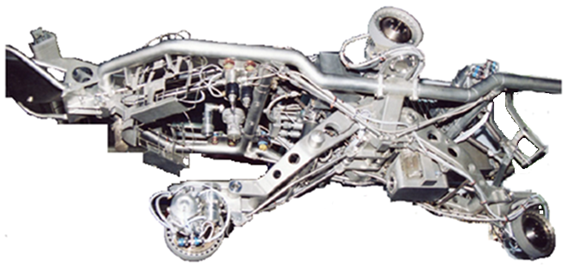
\includegraphics[width=.9\linewidth]{images/mir_01}
\end{center}
\end{minipage} \hfill
\begin{minipage}[c]{.7\linewidth}
Le robot MIR développé pour la vérification des cuves de Superphenix doit être adapté pour le contrôle d’une nouvelle génération de réacteurs à neutrons rapides.

L’objectif du robot MIR est de :
\begin{itemize}
\item assurer le contrôle surfacique télévisuel des soudures des deux cuves et des zones adjacentes ;
\item assurer le contrôle volumique par ultrasons des soudures de la cuve principale et des zones adjacentes. Une possibilité était offerte d’effectuer ce contrôle sur la cuve de sécurité ;
\item mesurer en permanence la distance entre les deux cuves.
\end{itemize}

\end{minipage} 

Le robot MIR est un véhicule motorisé composé d’un châssis tubulaire, de quatre bras articulés et des composants nécessaires à la mise en œuvre des contrôles et mesure. La structure est en acier inoxydable. La masse est d’environ 180 kg.

À l’extrémité de chaque bras, se trouve une roue motorisée en rotation et en direction. Il y a donc au total 4 roues qui servent d’appui contre les parois de cuve (principale et de sécurité).

Sur la partie inférieure, sont situés le mini bac d’inspection et son système de plaquage. Ce sous-ensemble constitue le dispositif d’inspection proprement dit. Le rôle dévolu au reste du robot étant de positionner le mini bac d’inspection au droit de la soudure à contrôler.
La chaîne d’énergie associée au déplacement
Chaque roue utilise un module de déplacement. Il y a quatre modules de déplacement sur le robot MIR, pilotant le déplacement.
Chaque module est composé d’un corps, d’une roue, du motoréducteur de traction, du motoréducteur d’orientation et du potentiomètre d’orientation.
La roue est la pièce tournante en contact avec les parois de la cuve. La surface extérieure torique est revêtue d’une couche mince de carbure de tungstène déposé par projection plasma. Ce revêtement est très tenace et présente l’avantage d’avoir un coefficient de frottement sur l’acier inoxydable élevé ($f \geq 0,5$).


\subsection{Étude de la fonction : Synchroniser les vitesses des roues}

On se place au niveau de l’arbre moteur avant réduction, couples et vitesses ramenées sur l’arbre moteur.

\begin{obj}
Synchroniser les vitesses des roues.
\end{obj}
La synchronisation automatique de la vitesse des quatre roues est basée sur la parfaite réversibilité de la transmission des efforts de la roue vers le réducteur puis le moteur. 

Ceci se concrétise par le fait que, pour une consigne de vitesse donnée, le contrôle-commande envoie la même tension aux bornes des quatre moteurs. La synchronisation s'effectue alors par les variations imposées au courant moteur. 

Par exemple si un motoréducteur a tendance à induire une vitesse supérieure à celle imposée par le déplacement de l'engin, cette tendance se traduit par un couple moteur plus grand, donc par une augmentation de l'intensité qui induit elle-même une diminution de la vitesse jusqu'à la valeur permise.

Ce principe qui permet un contrôle-commande relativement simple exige en contrepartie une réversibilité parfaite de fonctionnement du réducteur, toute dégradation de cette réversibilité entraînant rapidement un fonctionnement chaotique de l'engin.

Dans une première approche, on ne s’intéresse qu’aux roues inférieures \textbf{SA} et \textbf{SB}.

Les roues \textbf{SA} et \textbf{SB} sont munies des mêmes motoréducteurs avec les mêmes moteurs à courant continu.
Elles sont commandées en tension sur l’induit. Les circuits d’induit ont la même résistance $R$ et une inductance négligeable.

On s’intéresse d’abord au moteur de la roue \textbf{SA} seule.

On notera :
\begin{itemize}
\item $\omega_{mA}(t)$ : vitesse angulaire de rotation à la sortie du moteur, avant réduction (en $\text{rad}\text{s}^{-1}$);
\item $c_{mA}(t)$ : couple exercé par le moteur de la roue \textbf{SA} sur l’arbre moteur en N.m;
\item $c_{mB}(t)$ : couple exercé par le moteur de la roue \textbf{SB} sur l’arbre moteur en N.m;
\item $J$ : moment d’inertie équivalent en $\text{kg}{m}^2$.
\end{itemize}
Rappelons les équations régissant le moteur : 
\begin{itemize}
\item équations électriques (en négligeant l’effet de l’inductance) : $u(t)=Ri_A(t)+e_A(t)$;
\item équation mécanique issue de l’étude précédente, ramenée à l’arbre moteur de la roue \textbf{SA} : $c_{mA}(t)+c_{mB}(t)=J\dfrac{d\omega_{ma}(t)}{dt}$;
\item équations électromécaniques : $e_a(t)=K_A\omega_{mA}(t)$ et $c_{mA}(t)=K_Ai_A(t)$.
 \end{itemize}
 
L’entrée du système est la tension de commande appliquée aux bornes du moteur, la sortie est la vitesse de rotation de la roue \textbf{SA}, on peut modéliser le système à l’aide du schéma bloc suivant :
\begin{center}
	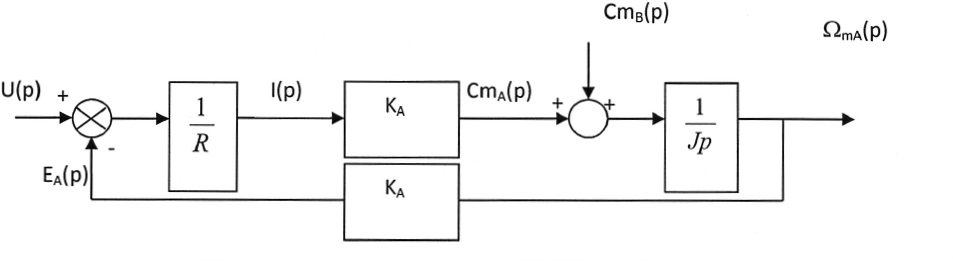
\includegraphics[width=\linewidth]{images/fig_10}
\end{center}



\subparagraph{}
\textit{Exprimer la fonction de transfert $\dfrac{\Omega_{mA}(p)}{U(p)}$ lorsque $C_{mB}(p)=0$ et la mettre sous forme canonique.}
\ifprof
\begin{corrige}
\end{corrige}
\else
\fi


\subparagraph{}
\textit{Exprimer quelle serait la valeur finale de la vitesse de rotation du moteur raccordé à la roue \textbf{SA}, notée $\omega_{mAf0}$ si on considère que $C_{mb}(p)=0$, et ceci pour une entrée modélisée par un échelon de tension d’amplitude $u_0$.}
\ifprof
\begin{corrige}
\end{corrige}
\else
\fi


\subparagraph{}
\textit{Exprimer la fonction de transfert $\dfrac{\Omega_{ma}(p)}{C_{mb}(p)}$ lorsque $U(p)=0$ et la mettre sous forme canonique.}
\ifprof
\begin{corrige}
\end{corrige}
\else
\fi

Si les deux roues fonctionnent à la même vitesse, on a la structure du schéma bloc de la figure 10 pour chacune des deux roues.

Mais si les moteurs ont une légère différence, par exemple la constante électromécanique $K_A$ et $K_B$, les 2 roues prendraient des vitesses différentes. Mais contraintes par le châssis et l’adhérence aux parois à tourner à la même vitesse (en ligne droite), elles exercent l’une sur l’autre un effort qu’on peut ramener à l’arbre moteur sous forme d’un couple supplémentaire $C_{mB}$ sur la roue \textbf{SA}, et $C_{mA}$ sur la roue \textbf{SB}. On a alors le schéma suivant :
\begin{center}
	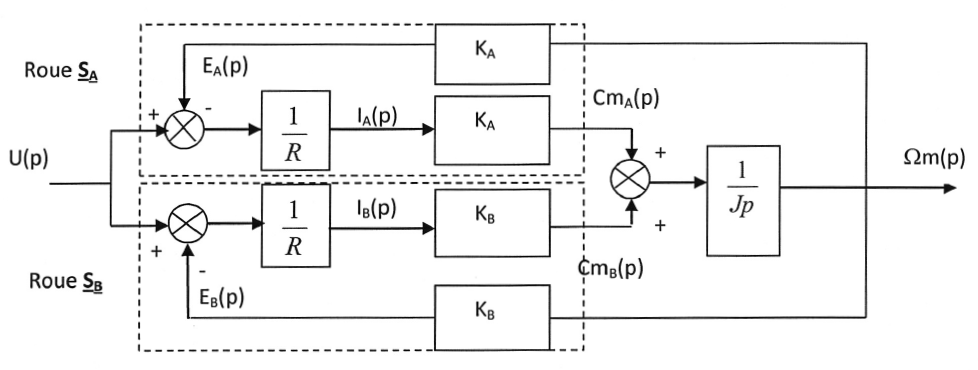
\includegraphics[width=\linewidth]{images/fig_11}
\end{center}

\subparagraph{}
\textit{Exprimer la fonction de transfert globale sous forme canonique : $\dfrac{\Omega_m(p)}{U(p)}$.}
\ifprof
\begin{corrige}
\end{corrige}
\else
\fi


\subparagraph{}
\textit{Si l’entrée est un échelon de tension d’amplitude $u_0$, calculer la valeur finale de la vitesse de rotation de chacun des moteurs, notée $\omega_\text{finale}$. Conclure quant à la possibilité d’avoir roulement sans glissement entre chacune des roues et les cuves.}
\ifprof
\begin{corrige}
\end{corrige}
\else
\fi

\section{Étude de la fonction Ft12 : Déplacer le transducteur à vitesse constante}

Le robot MIR étant à l’arrêt entre les deux cuves, le mini bac est plaqué contre la paroi de la cuve à contrôler. Pour l’inspection des soudures, le transducteur 13 (capteur de l’état des soudures) doit se déplacer à l’intérieur du mini bac d’inspection à vitesse constante. Le mini bac est rempli d’un fluide visqueux. L’inspection peut avoir lieu pour n’importe quelle position du robot MIR, donc l’angle $\alpha$ qui caractérise la direction du déplacement du transducteur par rapport à l’horizontale, est susceptible de prendre toute valeur comprise entre $-\pi/2$ (robot tête en bas) et $\pi/2$ (robot tête en haut). Afin de garantir la qualité des résultats de mesure, le transducteur doit donc se déplacer à une vitesse $V_0$ constante par rapport à la paroi, et ceci pour toute valeur de l’angle $\alpha$.

\begin{obj}
Qualifier la précision statique du système et définir les améliorations à apporter.
\end{obj}

\begin{center}
	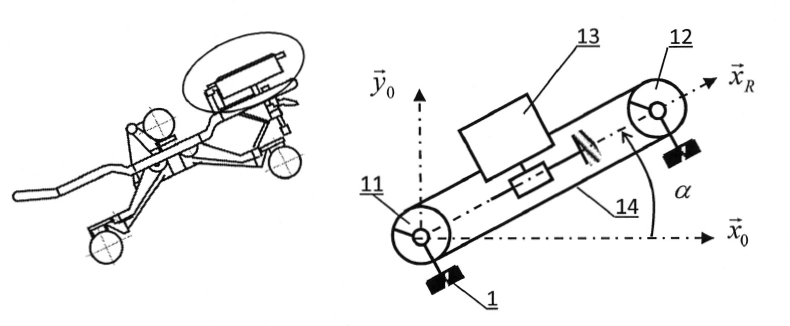
\includegraphics[width=\linewidth]{images/fig_12}
\end{center}

L’objectif de cette partie est de dimensionner le correcteur nécessaire au respect d’un écart statique nul, et ceci malgré le caractère variable de l’angle $\alpha$.

Le transducteur est en liaison glissière de direction $\vect{x_r}$, avec le corps \textbf{1} du robot MIR. La chaîne d’énergie est composée entre autre, d’un actionneur rotatif qui exerce un couple $c(t)$ sur le pignon \textbf{11}, qui est en liaison pivot, supposée parfaite, avec le robot MIR.
Un système poulies (\textbf{11} et \textbf{12}) et courroie crantée \textbf{14} impose le mouvement de translation au transducteur \textbf{13}.
 
 Le comportement dynamique du système est régit par l'équation suivante  
 $$
 M_{eq}\dfrac{dv_r(t)}{dt}=\delta c(t) + \beta v_r(t) + \gamma g
 $$

On cherche à garantir une vitesse de translation du transducteur \textbf{13} égale à la valeur de consigne indépendamment de l’angle $\alpha$.

Pour cela, on réalise le système bouclé suivant :

\begin{center}
	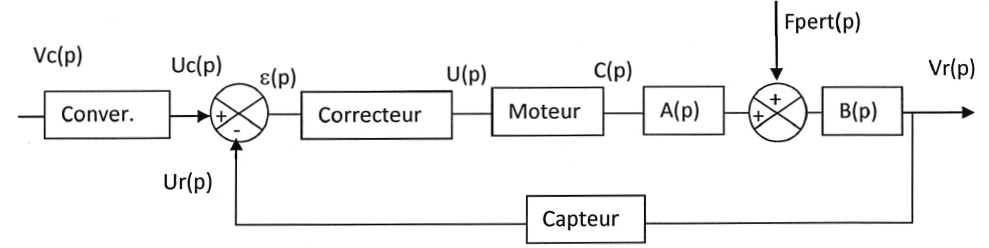
\includegraphics[width=\linewidth]{images/fig_13}
\end{center}

Notations : $V_r(p)$ est la transformée de Laplace de $v_r(t)$ vitesse de translation du transducteur \textbf{13}.
$F_{\text{pert}}(p)$ est la transformée de Laplace de $f_{\text{pert}}(t)$, avec :
$f_{\text{pert}}(t) = -m_t  \sin \alpha u(t)$ avec $u(t)$ échelon unitaire.


\subparagraph{}
\textit{En supposant des conditions initiales nulles, exprimer les fonctions de transfert $A(p)$ et $B(p)$ en fonction entre autres de $\delta$, $\beta$ et $M_{eq}$.
}
\ifprof
\begin{corrige}
\end{corrige}
\else
\fi

\vspace{.25cm}
Le capteur est modélisé par un gain pur de valeur $K_{capt}$.


\subparagraph{}
\textit{En supposant une perturbation nulle, quelle doit être la valeur du gain $K_{conv}$ du convertisseur modélisé par un gain pur, afin que l’écart $\varepsilon(t)$ soit nul quand la valeur de la vitesse réelle $v_r(t)$ est égale à la valeur de la consigne $v_c(t)$. 
}
\ifprof
\begin{corrige}
\end{corrige}
\else
\fi

\vspace{.25cm}
On adopte pour la suite la modélisation suivante :

\begin{center}
	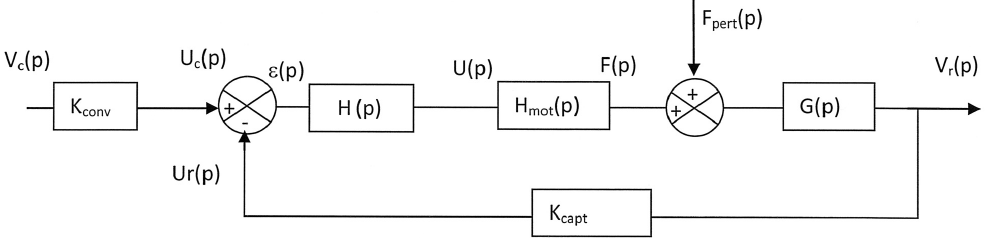
\includegraphics[width=\linewidth]{images/fig_14}
\end{center}

Avec $H_{mot}(p)=\dfrac{K_m}{1+\tau_m p}$, $G(p)=\dfrac{K}{1+\tau p}$ et $H(p)=K_{cor}$ fonction de transfert du correcteur.


\subparagraph{}
\textit{Exprimer les deux fonctions de transfert : $H_1(p)=\left(\dfrac{V_r(p)}{V_c(p)} \right)_{F_{\text{pert}}(p)=0}$ et $H_2(p)=\left(\dfrac{V_r(p)}{F_{\text{pert}}(p)} \right)_{V_c(p)=0}$. en fonction des gains $K_\text{conv}$, $K_{\text{cor}}$, et $K_{\text{capt}}$ ainsi que des fonctions de transfert $H_{\text{mot}}(p)$ et $G(p)$.}
\ifprof
\begin{corrige}
\end{corrige}
\else
\fi


\subparagraph{}
\textit{En supposant que $K_{\text{cor}}= 1$ et en indiquant les valeurs remarquables, tracer les diagrammes asymptotiques dans le plan de Bode de la fonction de transfert en boucle ouverte $\dfrac{U_r (p)}{\varepsilon(p)}$ en utilisant les valeurs numériques suivantes :}
$$
Kçm = \SI{0.1}{N.V^{-1}} 
\quad \tau_m= \SI{0,01}{s} 
\quad K_{\text{capt}} = \SI{50}{V.s.m^{-1}}
\quad K = \SI{200}{m.s^{-1}.N^{-1}}
\quad \tau = \SI{1}{s}
$$

\ifprof
\begin{corrige}
\end{corrige}
\else
\fi


\subparagraph{}
\textit{Déterminer le gain en décibel de la fonction de transfert en boucle ouverte (courbe réelle) pour la pulsation de \SI{100}{rad.s^{-1}}.}
\ifprof
\begin{corrige}
\end{corrige}
\else
\fi


On formule l’hypothèse simplificatrice suivante : la phase de la fonction de transfert en boucle ouverte pour une pulsation de 100 rad/s est de -135\degres.


\subparagraph{}
\textit{On souhaite une marge de gain \SI{12}{dB} et un marge de phase de 45\degres, en utilisant le résultat de la question précédente, déterminer la valeur numérique correspondante de $K_{\text{cor}}$.
Commenter la valeur de la marge de gain obtenue ?}
\ifprof
\begin{corrige}
\end{corrige}
\else
\fi


\subparagraph{}
\textit{On impose une vitesse constante en entrée de valeur $v_0$ ($v_c(t)=v_0.u(t)$) avec $u(t)$ fonction échelon unitaire de Heaviside. Exprimer l’écart statique en régime permanent en tenant compte de la perturbation (en fonction de l’angle $\alpha$, de la valeur de $K_{\text{cor}}$ et des données).}
\ifprof
\begin{corrige}
\end{corrige}
\else
\fi

\vspace{.25cm}

On souhaite obtenir une vitesse de translation indépendante de l’inclinaison. Pour toute la suite du sujet, on installe un correcteur intégral du type $\dfrac{K_c}{p}$, placé au début de la chaîne d’action.

\subparagraph{}
\textit{On impose de nouveau une vitesse constante en entrée de valeur $v_0$ ($v_c(t)=v_0.u(t)$); exprimer l’expression du nouvel écart statique en régime permanent (en fonction de l’angle $\alpha$ et des données). Pouvait-on prévoir ce résultat ?}
\ifprof
\begin{corrige}
\end{corrige}
\else
\fi


%
%\subparagraph{}
%\textit{}
%\ifprof
%\begin{corrige}
%\end{corrige}
%\else
%\fi
%
%
%
%\subparagraph{}
%\textit{}
%\ifprof
%\begin{corrige}
%\end{corrige}
%\else
%\fi

\end{document}

\begin{center}
	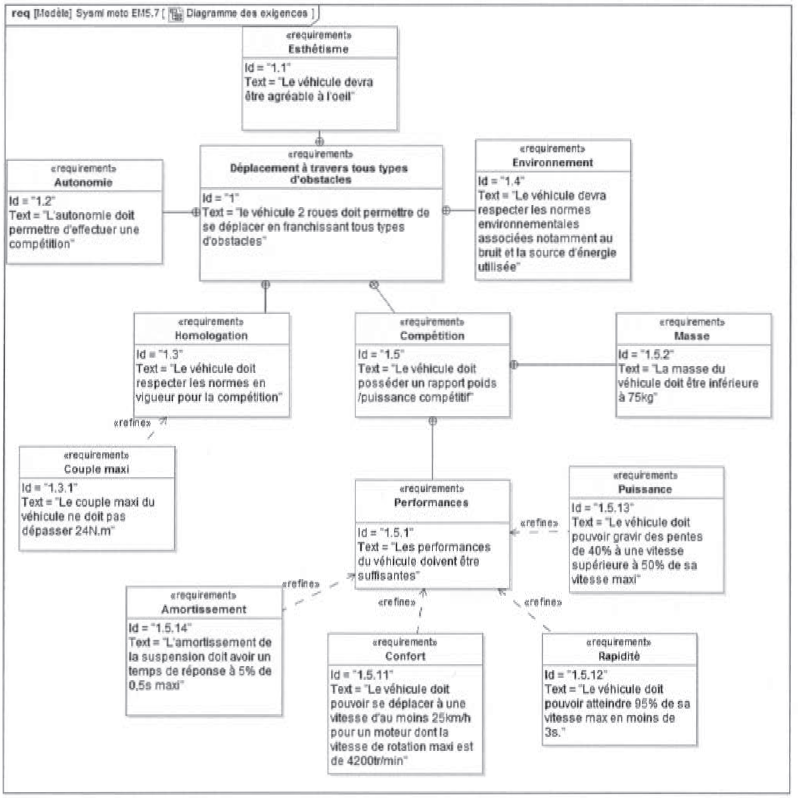
\includegraphics[width=\linewidth]{images/fig_02}
\end{center}

\begin{center}
	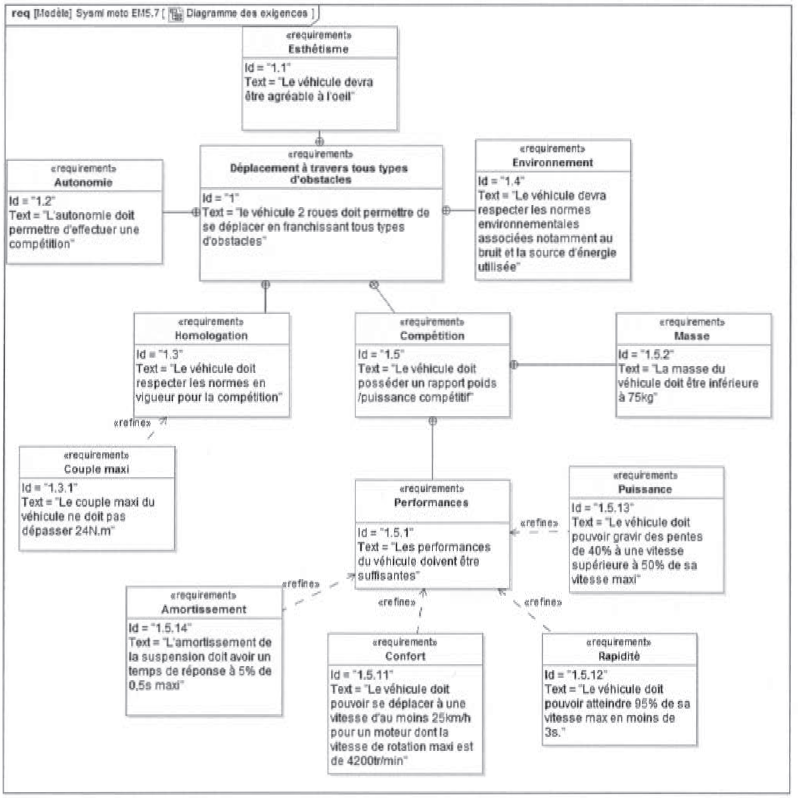
\includegraphics[width=\linewidth]{images/fig_02}
%\textit{Diagramme de Bode (gain uniquement) du système corrigé.}
\end{center}

\subparagraph{}
\textit{}
\ifprof
\begin{corrige}
\end{corrige}
\else
\fi
